\documentclass[electronics,article,submit,moreauthors]{Definitions/mdpi}
\usepackage{tabularx}
\usepackage{array}
\firstpage{1}
\pubvolume{1}
\issuenum{1}
\articlenumber{0}
\pubyear{2026}
\copyrightyear{2026}
\datereceived{}
\daterevised{}
\dateaccepted{}
\datepublished{}
\Title{Cross-Series Context for 24-Step-Ahead Point Forecasting of Multi-Region Power Load: A Matched Rolling-Origin Component Evaluation}
\Author{Jieyun Zheng, Linyao Zhang, Zhanghuang Zhang, Zhuolin Chen, Ying Shi}
\AuthorNames{Jieyun Zheng, Linyao Zhang, Zhanghuang Zhang, Zhuolin Chen, Ying Shi}
\address{Economic and Technological Research Institute of State Grid Fujian Electric Power Co., Ltd., Fuzhou 350000, Fujian, China}
\corres{Correspondence: zjy\_0701@163.com (J. Zheng)}
\abstract{Cross-correlated regional load series motivate graph and attention mechanisms, but fixed-split accuracy tables can confound cross-series information with head capacity and temporal selection. CSA-LoadNet combines a shared temporal encoder, cross-series attention, and a compact prediction head for scalar 24-position-ahead multi-region load forecasting. A historical ten-seed fixed split favored the full model over MLP and a smaller-head TemporalOnly ablation. We therefore ran a new immutable OPSD control study at eight quarterly rolling origins and five common seeds. The inferential unit is the rolling origin after averaging seeds. Every new arm has 29,815 parameters and the same 100--64--1 head, optimizer, epoch budget, seeds, and executed attention path. The proposed arm reaches mean origin-level MAPE 0.03664 and WAPE 0.03678, versus 0.03689 and 0.03711 for a target-only matched-context control; neither difference separates (MAPE Holm p = 0.984; WAPE raw p = 0.227). Uniform cross-series, Euclidean-distance, and learned-scale variants also remain unresolved after primary-family correction. A capacity-matched independent-encoder arm is worse, but its narrower per-series hidden layers and lower encoder arithmetic prevent attribution to sharing alone. Exact-hierarchy Ausgrid results remain adverse to the proposed forecaster. Thus the earlier aggregation attribution does not replicate under the capacity-matched rolling-origin estimand, and no tested weighting form is established as superior.}
\keyword{24-step-ahead point forecasting; multi-region load; cross-series attention; matched controls; rolling-origin evaluation; negative results; open power system data}
\providecommand{\tightlist}{\setlength{\itemsep}{0pt}\setlength{\parskip}{0pt}}
\begin{document}
\section{Introduction}\label{introduction}

At nominal hourly cadence, load forecasts made 24 processed positions in advance can inform operational planning. The experiment reported here predicts one value at lead 24 for each processed forecast origin; it does not produce the 24 hourly values of a next-day schedule, and complete-row filtering means a lead of 24 positions is not guaranteed to equal 24 elapsed UTC hours around a discarded row. In multi-region forecasting, such as countries in an interconnection or profile classes in a distribution network, the individual series share weather regimes, calendar structure, and economic rhythms. This raises a practical question: does cross-series information improve on forecasts constructed independently for each series?

Recent applied studies address this question with increasingly elaborate architectures. Graph convolutions, learned adjacency matrices, spatio-temporal attention stacks, and tensor decompositions have been combined with recurrent or transformer backbones, commonly with the complete architecture leading the reported accuracy table {[}1--4{]}.

A parallel line of evidence cautions against equating architectural complexity with forecast accuracy. Linear models outperform several transformer variants on standard long-horizon benchmarks {[}5{]}, statistical methods remain competitive in the M-competitions {[}6,7{]}, and methodological audits show that some reported gains shrink under stricter protocols {[}8{]}.

These findings leave a component-level question unresolved. Cross-series models are often evaluated as complete architectures, making it difficult to determine whether aggregation itself helps, whether a particular weighting geometry matters, and whether any gain persists across horizons and aggregation structures.

CSA-LoadNet is a compact neural forecaster in which a shared encoder processes each region's load history and cross-series attention aggregates the other encodings. Attention weights can use Poincar\'{e} distance with a fixed or learned inverse-temperature, Euclidean distance with the same scale convention, or equal averaging. The implementation does not make the metric curvature depend on this scale. Each mechanism is an independent switch.

The historical component matrix contains the full model and five single-switch ablations. Because its TemporalOnly arm also has a smaller head and all conclusions came from one split, the new confirmatory comparison narrows scope to OPSD lead 24 and introduces matched target-only, uniform-neighbor, Euclidean, fixed-scale, and independent-encoder controls at eight rolling origins. Five seeds are averaged within origin, and exact paired sign-flip tests use origin as the outer unit. The earlier targeted MLP and multi-dataset results remain contextual evidence rather than equal-strength confirmation.

The paper makes three contributions:

\begin{enumerate}
\def\labelenumi{\arabic{enumi}.}
\tightlist
\item
  \textbf{A capacity- and head-matched component design.} The new target-only and uniform-neighbor arms retain the complete 48-dimensional context slot, 100--64--1 head, 29,815 instantiated parameters, optimizer, seeds, epochs, and parameterized attention computation. They separate cross-series content from the smaller-head defect of the historical TemporalOnly switch.
\item
  \textbf{A temporally replicated analysis with an appropriate outer unit.} Eight quarterly OPSD origins are evaluated with five common seeds; MAPE is primary and WAPE secondary. Seeds are averaged within method--origin before exact paired inference, so neither hourly targets nor optimization runs are treated as independent temporal replications.
\item
  \textbf{A bounded negative component map.} The fixed-split aggregation signal does not separate from the matched target-only control across rolling origins. Learned Poincar\'{e} weighting does not separate from uniform or Euclidean cross-series context after correction, while the shared-versus-independent result remains confounded by hidden-width allocation. Historical short-horizon, SimBench, and exact-hierarchy results retain their adverse or unresolved scope.
\end{enumerate}

The paper is organized as follows. Section 2 reviews the three research threads the study draws on. Section 3 describes the datasets, tasks, and split protocol. Section 4 specifies CSA-LoadNet and its ablation switches. Section 5 details baselines, training, and statistics. Section 6 reports results, Section 7 interprets the setting-dependent component evidence, Section 8 states limitations, and Section 9 concludes.

\begin{center}\rule{0.5\linewidth}{0.5pt}\end{center}

\section{Related Work}\label{related-work}

Three threads frame this study: the deep-architecture lineage of short-term load forecasting, cross-series and graph-structured forecasting, and rigorous evaluations that compare complex forecasters with simple baselines. An extended review with full citation context accompanies the released evidence package.

\subsection{Deep Architectures for Short-Term and 24-Hour-Ahead Load Forecasting}\label{deep-architectures-for-short-term-and-24-hour-ahead-load-forecasting}

Recurrent networks were among the first deep models to displace classical load forecasters. Building on the LSTM cell {[}9{]}, Kong et al.~demonstrate short-term forecasting at the residential scale {[}10{]}. DeepAR extends shared training to large panels of related series {[}11{]}, an idea reflected in CSA-LoadNet's shared encoder. Temporal convolutional networks offer a lower-cost alternative {[}12{]}, while the Temporal Fusion Transformer {[}13{]} and Informer {[}14{]} extend attention-based forecasting.

Applied load forecasting increasingly uses hybrid models, including LSTM--CNN fusion {[}15{]}, BiLSTM--Transformer combinations {[}16{]}, decomposition pipelines {[}17{]}, and LSTM--XGBoost ensembles {[}18{]}. Evidence for the added component, however, is commonly limited to one accuracy table. Multi-seed distributions and component-level tests remain uncommon.

\subsection{Cross-Series and Graph-Structured Load Forecasting}\label{cross-series-and-graph-structured-load-forecasting}

A second thread exploits correlation among regional or nodal series. LSTNet models dependence through joint convolutional--recurrent channels {[}19{]}. Graph formulations emerged in traffic forecasting {[}20{]}, and MTGNN learns adjacency end to end {[}21{]}. Power-load examples include LoadSeer {[}4{]}, GCN--BiLSTM--Adaboost {[}1{]}, spatio-temporal graph transformers {[}2{]}, and GCN--Transformer integration {[}3{]}. A parallel literature treats multiple series as a hierarchy requiring reconciliation {[}22,23{]}, with Ausgrid as a common testbed {[}24{]}.

These graph-based studies propose increasingly elaborate weighting mechanisms. Their comparisons rarely test the selected weighting against equal averaging under an identical seeded protocol. Consequently, the contribution of aggregation can be conflated with that of its parameterization.

\subsection{Simple Baselines and Honest Evaluation}\label{simple-baselines-and-honest-evaluation}

The third thread concerns evaluation discipline. Sound out-of-sample practice was codified early {[}25{]}, and temporal leakage from naive cross-validation is well documented {[}26{]}. Common metrics also have known failure modes; MAPE becomes unstable near zero loads {[}27{]}, directly motivating the SimBench and Ausgrid choices. Diebold--Mariano testing {[}28{]} made statistical comparison a standard forecasting question. The M competitions {[}6,7{]}, DLinear {[}5{]}, and later best-practice guides {[}8{]} further emphasize strong simple baselines.

This evaluation literature mainly operates at whole-model granularity. The present study extends it to individual forecaster components, using multiplicity-corrected tests to determine which component claims survive. Section 6.3 applies that logic to the aggregation weight forms.

\begin{center}\rule{0.5\linewidth}{0.5pt}\end{center}

\section{Datasets, Tasks, and Split Protocol}\label{datasets-tasks-and-split-protocol}

\subsection{Datasets and Forecast Tasks}\label{datasets-and-forecast-tasks}

We evaluate on three public datasets chosen to span three distinct multi-series regimes: country-level national loads, distribution-system load profiles, and a customer/region/system hierarchy (Table 1).

\begin{table*}[t]
\centering
\footnotesize
\setlength{\tabcolsep}{3pt}
\caption{Datasets, series pools, and temporal splits (from \texttt{evidence/source/real\_opsd\_source\_profile.csv}, \texttt{evidence/source/real\_simbench\_source\_profile.csv}, and \texttt{src/configs/real\_ausgrid\_exact\_hierarchy\_v8\_config.json}).}\label{tab:1}
\begin{tabularx}{\textwidth}{@{}>{\raggedright\arraybackslash}X >{\raggedright\arraybackslash}X >{\raggedright\arraybackslash}X >{\raggedright\arraybackslash}X@{}}
\toprule
Property & OPSD & SimBench & Ausgrid \\
\midrule
Source & Open Power System Data, 60 min single-index time series [29] & SimBench complete mixed dataset, \texttt{LoadProfile.csv} [30] & Ausgrid solar-home half-hourly data [24] \\
Series pool & 6 country loads: DE, FR, IT, ES, NL, PL & 8 profiles: BL-H, G0-A, G0-M, G1-A, G1-B, G1-C, G2-A, G3-A & Exact 17-node hierarchy: 12 named customer leaves, four sums of postcode-sorted three-leaf groups, and their exact system sum \\
Processed period & 2015-01-01T01:00:00Z to 2018-12-31T01:00:00Z; first 35,000 retained hourly rows & 01.01.2016 00:45 to 30.12.2016 23:45; first 8760 constructed hourly rows & 2010-07 to 2013-06; 26,304 constructed hourly rows \\
Forecast-origin boundary & index 24,500 = 2017-10-19T03:00:00Z & index 6132 = 12.09.2016 13:45 & index 18,412 (70\% of 26,304) \\
Point leads & 1 and 24 processed positions & 1 and 24 processed positions & 24 constructed positions \\
Primary metric & MAPE & normalized MAE & sMAPE \\
\bottomrule
\end{tabularx}
\end{table*}

For every dataset and lead \(h\), a sample is \((X_{t-167:t},y_{i,t+h})\): the model sees the inclusive 168-position history ending at origin index \(t\) and predicts one scalar for target series \(i\). Origins advance by one processed row. Thus the \(h=24\) experiment is \textbf{24-step-ahead point forecasting}, not direct or recursive prediction of a 24-value next-day trajectory. In the historical fixed split, the origin boundary is \(b=\lfloor0.7n\rfloor\): training origins satisfy \(168\leq t<b\), test origins satisfy \(b\leq t<n-h\), training labels end at \(b+h-1\), and test labels start at \(b+h\). Evaluation targets do not overlap, although historical training labels cross the origin boundary. The new rolling-origin experiment instead requires every training target to precede its test-origin boundary.

\textbf{OPSD cleaning and time contract.} The parser reads \texttt{utc\_timestamp} and the six named \texttt{*\_load\_actual\_entsoe\_transparency} columns. It retains a row only when all six cells are nonempty and parse as floating-point values, drops the entire row otherwise, and stops after 35,000 retained rows; it performs no interpolation or imputation. The retained-row count is recorded, but the number and location of discarded source rows are not, and hourly continuity is not revalidated after filtering. Timestamps carry \texttt{Z} and remain in UTC, so no duplicated or missing local daylight-saving hour is introduced and no country-local conversion is applied.

\textbf{SimBench cleaning, aggregation, and time contract.} The parser selects the first eight header fields ending in \texttt{\_pload}, skips a 15-minute source row if any selected value fails numeric parsing, and takes the unweighted arithmetic mean of each successive four retained rows. The constructed hour is labeled by the fourth source row (for example, the first label is \texttt{00:45}); values are means, not energy sums. No interpolation is applied, and a discarded quarter-hour can cause a four-valid-row block to span a source-time gap. The source labels have no timezone field in the inspected profile or parser. They are kept as naive labels, with no daylight-saving conversion, and processing stops after 8760 constructed hours.

\textbf{Ausgrid cleaning, aggregation, and time contract.} Only \texttt{GC} rows from the three annual files are used. Each pair of adjacent half-hour cells is summed to one hourly value; an empty half-hour cell is replaced by zero, whereas a malformed or short daily row is skipped. Dates are parsed in one of three declared day-month-year formats and checked for one-day contiguity. The processor creates the naive label \texttt{YYYY-MM-DDTHH:00} for slot pair \((2H,2H+1)\); it records no timezone and forces 24 constructed hourly slots per date, so no daylight-saving repeated or skipped hour is represented. Customers 134, 104, 255, 141, 228, 147, 55, 131, 21, 82, 58, and 109 are the leaves. \texttt{region1} sums \{82, 147, 255\}, \texttt{region2} sums \{228, 109, 131\}, \texttt{region3} sums \{134, 141, 55\}, \texttt{region4} sums \{21, 58, 104\}, and \texttt{system\_total} sums all 12 leaves. These are deterministic postcode-sorted groups, not claims that every leaf in a group has the same postcode.

The Ausgrid structural filter is not train-only: the code first keeps the 299 customers having the maximum observed day count over the full three-year record and then selects the 12 highest total-energy customers using that full record. This uses future-period availability and energy for leaf selection. It does not expose test targets to model fitting or reconciliation, but it can favor continuously observed, high-consumption leaves and is retained as a data-visibility limitation. No result here is presented as evidence from a train-only leaf-selection design.

\subsection{Primary Metrics and Why They Differ per Dataset}\label{primary-metrics-and-why-they-differ-per-dataset}

The primary metric is chosen per dataset to avoid known metric pathologies {[}27{]}. For a fixed dataset--horizon test set of \(N\) targets, the implementation computes

\[
\operatorname{MAPE}=\frac{1}{N}\sum_{j=1}^{N}\frac{|y_j-\hat y_j|}{\max(\epsilon,|y_j|)},
\]

\[
\operatorname{nMAE}=\frac{N^{-1}\sum_{j=1}^{N}|y_j-\hat y_j|}
{\max\!\left(\epsilon,\max_j y_j-\min_j y_j\right)},
\]

and

\[
\operatorname{sMAPE}=\frac{1}{N}\sum_{j=1}^{N}
\frac{2|y_j-\hat y_j|}{\max(\epsilon,|y_j|+|\hat y_j|)},
\]

and the new OPSD secondary metric is

\[
\operatorname{WAPE}=\frac{\sum_{j=1}^{N}|y_j-\hat y_j|}{\max(\epsilon,\sum_{j=1}^{N}|y_j|)}.
\]

All denominators use \(\epsilon=10^{-6}\). The normalization range in nMAE is computed once from the common test targets; it is an evaluation scale and is identical for all methods, not a training input. Country-level OPSD loads are strictly positive and far from zero, so MAPE is interpretable there; WAPE supplies a scale-aggregated secondary check. SimBench profile values approach zero at many timestamps, where MAPE denominators become unstable; SimBench methods are therefore ranked by nMAE and MAPE is retained descriptively.

For the exact Ausgrid hierarchy, let \(\bar s_L\), \(\bar s_R\), and \(s_T\) be the mean node sMAPE over the 12 leaves, the four regions, and the root. The predeclared primary metric gives each level equal weight rather than letting 12 leaves dominate:

\[
\operatorname{HWSMAPE}=\frac{\bar s_L+\bar s_R+s_T}{3}.
\]

With bottom-level forecast matrix \(\hat{B}\) and summing matrix \(S\in\{0,1\}^{17\times12}\), structural coherence requires \(\hat{Y}=S\hat{B}\). We report the scale-normalized violation

\[
C(\hat Y)=\frac{1}{5T}\sum_{i=13}^{17}\sum_{t=1}^{T}
\frac{|\hat y_{it}-(S\hat B)_{it}|}{\max(\epsilon,T^{-1}\sum_t|y_{it}|)}.
\]

Bottom-up, top-down, and OLS projection reconciliation are evaluated separately from forecasting accuracy. All significance tests in Section 6 use the primary metric of the respective dataset; secondary metrics, including MAE, RMSE, level-specific sMAPE, peak-load error, and coherence violation, are preserved in the evidence tables.

\subsection{Temporal Protocol and Train-Only Operations}\label{temporal-protocol-and-train-only-operations}

Forecasting comparisons are sensitive to temporal leakage {[}8,26{]}. The sample origins are not shuffled across the train/test boundary. Per-series z-normalization means and sample standard deviations (\texttt{torch.std} with correction 1, clamped below at \(10^{-6}\)) are computed from raw values at indices \([0,b)\); this pre-test segment includes the later validation portion and is therefore a \textbf{training-segment}, not fit-subset, transformation. The final 15\% of strided training origins by time is used to choose the lowest-validation-loss checkpoint. All test origins are evaluated without stride.

The new identifiable experiment adds eight quarterly OPSD rolling origins at \texttt{2017-01-01}, \texttt{2017-04-01}, \texttt{2017-07-01}, \texttt{2017-10-01}, \texttt{2018-01-01}, \texttt{2018-04-01}, \texttt{2018-07-01}, and \texttt{2018-10-01} UTC. Each origin evaluates the next 672 processed origins (nominally 28 days), with six target-series forecasts per origin and no test stride. Training origins use stride 3 and must have their lead-24 target strictly before the rolling origin. Normalization is recomputed from rows strictly before each origin, the last 15\% of eligible strided origins supplies validation, and all eight epochs are completed before the lowest-validation-loss checkpoint is restored. The parser scanned 35,043 source rows, discarded 43 rows missing at least one selected country value, and retained the frozen first 35,000 valid rows. Consequently, ``24 h'' in the historical terminology is exactly a 24-processed-position lead but can differ from 24 elapsed UTC hours around a discarded row; the new analysis retains target UTC dates for audit.

The cyclic covariates are derived from array position rather than parsed civil time: \texttt{hour\ =\ (t+h)\ mod\ 24} and \texttt{day-of-week\ =\ floor((t+h)/24)\ mod\ 7}, each encoded by sine and cosine. They should therefore be read as sequence-phase features. The implementation neither localizes timestamps nor supplies holidays or daylight-saving indicators. For reconciliation, only the top-down leaf proportions are fitted, using leaf energy at indices \([0,b)\); bottom-up uses no fitted proportions and OLS depends only on the fixed summing matrix. Dataset row-validity filtering occurs before the split, and the full-record Ausgrid structural selection is the exception disclosed above. These distinctions replace a blanket leakage-free claim.

\begin{center}\rule{0.5\linewidth}{0.5pt}\end{center}

\section{CSA-LoadNet}\label{csa-loadnet}

Figure 1 gives the complete forecasting path. Load histories enter the shared temporal encoder; target and context series are related only inside the cross-series attention block; and the target encoding, context vector, and sequence-phase features enter the prediction head. The three weight forms shown under the attention block are controlled alternatives evaluated with the same downstream network.

\begin{figure*}[t]
\centering

\includegraphics[width=0.94\textwidth]{figures/fig_architecture.png}
\caption{CSA-LoadNet data and model flow. The lower strip identifies independent evaluation datasets; it is not an input path. Poincare, Euclidean, and equal-weight attention share the same encoder, fusion, head, and training protocol.}\label{fig:1}
\end{figure*}

CSA-LoadNet (Cross-Series Attention Load Forecasting Network) is intentionally small: a shared temporal encoder, one cross-series attention block, and a compact prediction head. The design goal is not architectural novelty for its own sake but a testbed in which every mechanism is an independent switch, so that the component analysis of Section 6.2--6.3 attributes effects cleanly.

\textbf{Formal definitions.} For series \(i\), the 168-position history is standardized with statistics from the pre-test training segment \([0,b)\), including the validation portion,

\[
\tilde x_{i,t-\ell}=\frac{x_{i,t-\ell}-\mu_i^{\mathrm{train}}}{\max(\sigma_i^{\mathrm{train}},10^{-6})},
\qquad \ell=0,\ldots,167.
\]

The shared two-layer encoder is

\[
h_i=W_2\,\phi(W_1\tilde X_{i,t}+b_1)+b_2,\qquad
W_1\in\mathbb R^{96\times168},\; W_2\in\mathbb R^{48\times96},
\]

where \(\phi\) is ReLU. When Poincar\'{e} weighting is enabled, raw embeddings are projected inside a radius-0.95 unit ball and their fixed-curvature unit-ball distance is

\[
\bar e_i=0.95\,\frac{\tanh(\|e_i\|_2)}{\max(\|e_i\|_2,\epsilon)}e_i,\qquad
d_{\mathbb B}(\bar e_i,\bar e_j)=
\operatorname{arcosh}\!\left(1+
2\frac{\|\bar e_i-\bar e_j\|_2^2}
{(1-\|\bar e_i\|_2^2)(1-\|\bar e_j\|_2^2)}\right).
\]

The Euclidean control replaces \(d_{\mathbb B}\) by \(\|\bar e_i-\bar e_j\|_2\), and the equal-neighbor control fixes \(\alpha_{ij}=1/(m-1)\). For either learned-distance control, the per-target score scale is \(\tau_i=\operatorname{softplus}(\kappa_i)+0.1\) and \(\alpha_{ij}=\operatorname{softmax}_{j\ne i}[-\tau_i d(\bar e_i,\bar e_j)]\). Because \(\tau_i\) multiplies a metric whose curvature is otherwise fixed, it is an inverse-temperature or distance-scale parameter, not curvature. For any weight form, context fusion is

\[
g_i=\sum_{j\ne i}\alpha_{ij}W_vh_j,\qquad
u_i=[h_i\|g_i\|\operatorname{cal}(t+h)] .
\]

The prediction head and empirical training risk are

\[
\hat y_{i,t+h}=w_o^\top\phi(W_ou_i+b_o)+b_y,
\]

\[
\mathcal L_h(\Theta)=\frac{1}{|\mathcal T_{\mathrm{fit}}|m}
\sum_{t\in\mathcal T_{\mathrm{fit}}}\sum_{i=1}^{m}
\left(\tilde y_{i,t+h}-\hat y_{i,t+h}\right)^2 .
\]

With \(m\) series, embedding width \(d_e\), and temporal width \(d_h\), the cross-series block costs \(O(m^2d_e+m^2d_h)\) per batch item; the TemporalOnly ablation removes the quadratic terms. This complexity statement concerns the implemented dense pool, not sparse graph attention.

\subsection{Shared Temporal Encoder}\label{shared-temporal-encoder}

For each series \(i\) in the pool, the past 168 processed positions of per-series z-normalized load are passed through a shared multilayer perceptron \(168 \to 96 \to 48\), yielding a temporal encoding \(h_i \in \mathbb{R}^{48}\). Sharing one encoder across all series follows the cross-learning principle established by panel forecasters such as DeepAR {[}11{]}: every series' history contributes gradient signal to the same temporal features. The evaluated pool sizes are 6, 8, and 17 series.

Because the manuscript retains the shared-encoder construction, the new OPSD study also instantiates a parameter-matched independent-encoder control. Its six series-specific encoders use hidden widths 16, 16, 16, 16, 15, and 15 plus an effective 194-parameter calibration, yielding the same 29,815 total parameters and the same downstream head as the shared arm. This equality does not make the control compute-matched: its estimated encoder multiply-accumulate count per unique origin is 20,304 rather than 124,416, and the narrower per-series hidden layers change width allocation. The comparison therefore probes the combined sharing/width allocation, not sharing alone.

\subsection{Cross-Series Attention Aggregation}\label{cross-series-attention-aggregation}

Each series additionally owns a learned embedding \(e_i \in \mathbb{R}^{8}\). To forecast target series \(i\), the module computes attention weights over the other series in the pool,

\[
\alpha_{ij} = \frac{\exp\!\big(-\tau_i \, d(\bar e_i, \bar e_j)\big)}{\sum_{k \neq i} \exp\!\big(-\tau_i \, d(\bar e_i, \bar e_k)\big)},
\]

and aggregates their value-mapped temporal encodings into a context vector \(g_i = \sum_{j \neq i} \alpha_{ij} \, W_v h_j\). In the default configuration, \(d(\cdot,\cdot)\) is the fixed unit-ball Poincar\'{e} distance and \(\tau_i = \mathrm{softplus}(\kappa_i) + 0.1\) is a per-target learnable inverse-temperature. The code variable and archived ablation label use \texttt{kappa} and \texttt{FixedCurvature}, respectively, but no curvature-dependent metric is implemented. The Poincar\'{e} parameterization is one interchangeable option for producing \(\alpha_{ij}\). Section 6.3 shows that it is statistically inseparable from Euclidean-distance and equal weights; accordingly, no geometric property is claimed as a contribution. The component under test is the aggregation step itself: whether \(g_i\) should exist at all.

\subsection{Prediction Head and Sequence-Phase Features}\label{prediction-head-and-sequence-phase-features}

The prediction head concatenates the target encoding, aggregated context, and the four sequence-phase covariates defined in Section 3.3. A hidden layer of width 64 maps this vector to the scalar h-step-ahead prediction: \(\hat{y}_{i,t+h} = \mathrm{MLP}_{64}\big([\,h_i \,\|\, g_i \,\|\, \mathrm{phase}(t+h)\,]\big)\). The exact instantiated parameter counts are reported in Section 5.1; the proposed configuration is close to, but not equal to, the MLP baseline's capacity.

\subsection{Ablation Switches}\label{ablation-switches}

Five single-switch variants isolate each mechanism (configuration keys from \texttt{src/configs/real\_hyg\_neural\_config.json}):

\begin{itemize}
\tightlist
\item
  \textbf{TemporalOnly} (\texttt{no\_graph}): removes the aggregation module entirely; the head sees only \(h_i\) and the four sequence-phase features. This is the switch that tests whether cross-series aggregation contributes at all.
\item
  \textbf{Euclidean weights} (\texttt{euclidean}): replaces the Poincar\'{e} distance with Euclidean distance in the same weight formula.
\item
  \textbf{Equal-weight neighbors} (\texttt{equal\_neighbors}): replaces learned attention with uniform averaging over the pool.
\item
  \textbf{Fixed distance scale} (\texttt{fixed\_curvature}, historical key): sets \(\tau_i=1\) instead of learning it; it does not change metric curvature.
\item
  \textbf{No sequence-phase features} (\texttt{no\_calendar}, historical key): removes the four cyclic index features from the head.
\end{itemize}

The middle three switches jointly probe the \emph{form} of the aggregation weights; TemporalOnly probes the \emph{existence} of aggregation; the historical NoCalendar switch probes the orthogonal sequence-phase channel.

The new rolling-origin namespace adds controls that repair the historical head mismatch. \textbf{TargetSelfContext-Matched} replaces the neighbor aggregate presented to the head with the value-mapped target encoding; \textbf{UniformCrossSeries-Matched} averages the other five encoded series. Both retain the 48-dimensional context slot, 100--64--1 head, all 29,815 instantiated parameters, and the complete parameterized distance/attention path as a zero-weight audit computation. Euclidean and fixed-scale controls use the same head and capacity. These controls match the declared optimization, seed, epoch, batch, and executed parameterized computation budget; they do not claim identical wall-clock timing.

\subsection{Weighting Variants and Artifact Labels}\label{weighting-variants-and-artifact-labels}

The implementation exposes Poincar\'{e}, Euclidean, equal-weight, fixed-scale, and learnable-scale weighting variants through the ablation switches defined above. The empirical question is whether cross-series aggregation contributes and, separately, whether any tested weighting form is distinguishable. Archived files retain two historical labels: \texttt{HyG-LoadFormer\ (neural)} maps one-to-one to CSA-LoadNet, and \texttt{Ablation-FixedCurvature\ (neural)} maps to the fixed-distance-scale control \(\tau_i=1\). These labels document provenance and are not descriptions of a curvature-dependent metric.

\begin{center}\rule{0.5\linewidth}{0.5pt}\end{center}

\section{Experimental Setup}\label{experimental-setup}

\subsection{Methods Compared}\label{methods-compared}

Table 2 lists the implemented capacities. Counts are exact source-level arithmetic over instantiated tensors, including the embedding, scale, and value-map tensors that remain instantiated in TemporalOnly even though its forward pass does not use aggregation. The five external baselines span MLP, LSTM {[}9,10{]}, TCN {[}12{]}, DLinear {[}5{]}, and a lightweight two-layer patch transformer. All models consume the same 168-position normalized histories, split boundaries, and full test origins; they do not have identical parameter counts or epoch budgets.

\begin{table*}[t]
\centering
\scriptsize
\setlength{\tabcolsep}{3pt}
\caption{Methods and roles.}\label{tab:2}
\begin{tabularx}{\textwidth}{@{}>{\raggedright\arraybackslash}X >{\raggedright\arraybackslash}X >{\raggedright\arraybackslash}X >{\raggedright\arraybackslash}X@{}}
\toprule
Method & Role and implemented capacity & Instantiated parameters for pools $m=6/8/17$ & Max epochs (OPSD--SimBench / Ausgrid) \\
\midrule
CSA-LoadNet & shared 168--96--48 encoder; $m\times8$ embeddings; $m$ scales; 48--48 value map; 100--64--1 head & 29,815 / 29,833 / 29,914 & 15 / 10 \\
Euclidean weights; Equal-weight neighbors; Fixed distance scale & same modules as CSA-LoadNet; one weight-form switch & 29,815 / 29,833 / 29,914 & 15 / 10 \\
TemporalOnly & aggregation omitted from forward pass; 52--64--1 head; unused aggregation tensors remain instantiated & 26,743 / 26,761 / 26,842 & 15 / 10 \\
No sequence-phase features & aggregation retained; 96--64--1 head & 29,559 / 29,577 / 29,658 & 15 / 10 \\
TargetSelfContext-Matched; UniformCrossSeries-Matched & OPSD-only new controls; same shared encoder, context width, head, instantiated tensors, and parameterized forward path as CSA-LoadNet & 29,815 & 8 rolling-origin epochs \\
Independent-encoder control & six narrower series-specific encoders plus calibration; same context block, head, and total capacity, but lower encoder arithmetic & 29,815 & 8 rolling-origin epochs \\
MLP & 172--128--64--1; targeted after the preliminary screen & 30,465 & 20 / 20 \\
LSTM & one layer, scalar input, hidden width 48; 52--1 head & 9,845 & 6 / 6 \\
TCN & seven width-32 causal blocks, kernel 3, dilations 1--64; 36--1 head & 18,853 & 10 / 10 \\
DLinear & moving-average kernel 25; separate 168--1 trend and seasonal maps & 338 & 20 / 20 \\
PatchTST-lite & patch 16, stride 8, 20 patches; width 64, four heads, feed-forward width 128, two encoder layers & 70,597 & 8 / 8 \\
\bottomrule
\end{tabularx}
\end{table*}

\subsection{Training Protocol and Hyperparameter Disclosure}\label{training-protocol-and-hyperparameter-disclosure}

Table 3 discloses the recorded training settings. Architectures are fixed across datasets in the inspected source. The targeted ten-seed MLP comparison was selected after a preliminary three-seed architecture screen on the same fixed test trajectory, so it is not represented as comparator selection made without test visibility.

\begin{table*}[t]
\centering
\scriptsize
\setlength{\tabcolsep}{3pt}
\caption{Full hyperparameter disclosure (from \texttt{src/configs/real\_hyg\_neural\_config.json} and \texttt{src/configs/real\_p2\_v7\_config.json}).}\label{tab:3}
\begin{tabularx}{\textwidth}{@{}>{\raggedright\arraybackslash}X >{\raggedright\arraybackslash}X@{}}
\toprule
Setting & Value \\
\midrule
Lookback window & 168 h \\
Temporal encoder & shared MLP 168 $\rightarrow$ 96 $\rightarrow$ 48 \\
Series embedding dimension & 8 \\
Inverse-temperature / distance scale & $\tau_i=\mathrm{softplus}(\kappa_i) + 0.1$, learnable per target; the historical FixedCurvature control sets $\tau_i=1$ \\
Head & concat[target encoding, aggregated context, four sequence-phase values] $\rightarrow$ 64 $\rightarrow$ 1 \\
Optimizer / loss & Adam, lr $10^{-3}$ / MSE on per-series z-normalized targets \\
Batch size & 512 \\
Epochs & model-specific maxima in Table 2; every epoch is run and the lowest-validation-loss checkpoint is restored \\
Training-sample stride & OPSD/SimBench: 3 for every model. Ausgrid: 6 for CSA variants, 3 for external baselines. Test origins are never strided \\
Checkpoint selection & validation = final 15\% of strided training origins by time; best-validation state restored after the fixed epoch budget \\
Seeds (decision set) & 10: \{11, 23, 47, 59, 71, 83, 97, 109, 127, 139\} \\
Seeds (exact Ausgrid hierarchy) & same 10 seeds for every proposed, ablation, and baseline model \\
Reconciliation & independent base forecasts, Bottom-Up, training-proportion Top-Down, and unweighted OLS projection; fully defined in Section 6.4 \\
Hardware / framework & CPU for OPSD/SimBench; RTX 3090 with PyTorch 2.13.0+cu130 for the v8 Ausgrid rerun \\
\bottomrule
\end{tabularx}
\end{table*}

\textbf{Comparability statement.} Every model shares the origin split, training-segment normalization, four sequence-phase inputs where the architecture uses them, Adam learning rate, MSE objective, batch size, seed list for the decision comparisons, and complete test origins. Capacity and epoch budgets differ as disclosed in Table 2. On OPSD and SimBench every trained model uses stride 3. On Ausgrid all eleven models use the same GPU execution path and ten seeds, but CSA variants use stride 6 while external baselines use stride 3. The v8 CSV \texttt{train\_samples} field writes the stride-6 count for every method even though the baseline routine internally retains stride 3; it must not be used to claim equal training exposure. Runtime values are interpreted only within datasets. This asymmetry weakens causal attribution of the Ausgrid model ranking but does not reverse the reported adverse point estimates.

In the new OPSD namespace, the six component arms use five common seeds \{11, 23, 47, 59, 71\}, batch size 2048, eight completed epochs, manual eager Adam with the standard \(\beta_1=0.9\), \(\beta_2=0.999\), and \(\epsilon=10^{-8}\) equations, and a single RTX 3090. Manual Adam is used because the preserved PyTorch optimizer wrapper imports unavailable \texttt{sympy}; the algorithm and frozen hyperparameters are recorded in the immutable driver. Global deterministic-algorithm enforcement was unavailable for the same dependency reason, while fixed CPU/CUDA seeds, deterministic cuDNN, disabled cuDNN benchmarking, and \texttt{CUBLAS\_WORKSPACE\_CONFIG=:4096:8} were retained. The matched shared-encoder arms have equal parameters, heads, optimizer steps, data exposure, and executed parameterized paths. The independent-encoder arm has equal parameters but not equal encoder arithmetic.

\subsection{Statistical Methodology}\label{statistical-methodology}

The new confirmatory family is frozen to five OPSD lead-24 contrasts: CSA-Poincar\'{e}-Shared against target-self context, uniform cross-series context, Euclidean weighting, fixed scale, and the independent-encoder control. For method \(a\), rolling origin \(o\), and seed \(s\), let \(e_{aos}\) denote error. The seed runs are first averaged within origin,

\[
\bar e_{ao}=\frac{1}{5}\sum_{s=1}^{5}e_{aos},
\]

and inference uses the eight paired origin differences \(d_o=\bar e_{\mathrm{CSA},o}-\bar e_{b,o}\). The exact two-sided sign-flip p-value enumerates all \(2^8\) sign assignments to the mean of \(d_o\). Holm adjustment covers the five MAPE contrasts. Pointwise 95\% percentile intervals use 20,000 deterministic resamples of the eight origins. WAPE is the frozen secondary metric and is reported with unadjusted sign-flip p-values; MAE, RMSE, and sMAPE are descriptive. No equivalence margin was specified. Forecast hours, target series, days, and seeds are therefore not promoted to independent inferential replicates.

The historical fixed-split set--CSA-LoadNet, its five ablations, and MLP--was run for ten seeds per dataset/horizon on OPSD and SimBench. Each block contains six proposed-versus-opponent comparisons. On the corrected Ausgrid hierarchy, all eleven models use the same ten seeds under four reconciliation regimes. Those earlier analyses use two-sided Mann--Whitney U tests with Holm correction and seed-paired sign-flip sensitivity tests. They remain useful scope and baseline context, but the new rolling-origin matched family governs the aggregation-existence claim.

For reproducibility, let \(e_{a,s}\) be the primary error of method \(a\) at seed \(s\). The reported mean and dispersion are

\[
\bar e_a=\frac{1}{n_a}\sum_{s=1}^{n_a}e_{a,s},\qquad
s_a=\sqrt{\frac{1}{n_a-1}\sum_{s=1}^{n_a}(e_{a,s}-\bar e_a)^2}.
\]

For a proposed--baseline comparison with rank sum \(R_1\), the Mann--Whitney statistic is

\[
U_1=n_1n_2+\frac{n_1(n_1+1)}{2}-R_1,\qquad
U=\min(U_1,n_1n_2-U_1).
\]

If \(p_{(1)}\leq\cdots\leq p_{(m)}\) are the ordered raw p-values within one dataset--horizon family, the monotone Holm-adjusted values used in Figure 3 are

\[
p^{\mathrm{Holm}}_{(i)}=
\max_{1\leq j\leq i}\min\!\left(1,(m-j+1)p_{(j)}\right).
\]

The seed-paired descriptive effect in Figure 6 is computed only when the same seeds exist for both methods,

\[
\Delta_s=100\,\frac{e_{b,s}-e_{a,s}}{e_{b,s}},
\]

so positive values favor CSA-LoadNet. This percentage is an effect display, not the test statistic. No pair with unequal seed support is promoted to a paired inferential comparison.

\begin{center}\rule{0.5\linewidth}{0.5pt}\end{center}

\section{Results}\label{results}

\subsection{Capacity-Matched Rolling-Origin Control}\label{capacity-matched-rolling-origin-control}

Table 4 reports the new OPSD lead-24 comparison. Each entry is first averaged across five seeds within a rolling origin and then summarized across the eight origins. CSA-Poincar\'{e}-Shared has mean MAPE 0.036640 and WAPE 0.036775. TargetSelfContext-Matched has MAPE 0.036894 and WAPE 0.037109. The proposed-minus-control differences are -0.000253 MAPE (pointwise origin-bootstrap 95\% interval {[}-0.000669, 0.000232{]}, raw exact p = 0.328, Holm p = 0.984) and -0.000334 WAPE ({[}-0.000778, 0.000153{]}, raw p = 0.227). Six of eight origin means favor the proposed arm on MAPE, but the comparison does not separate. The historical aggregation attribution is therefore not confirmed by the capacity- and head-matched rolling-origin estimand.

\begin{table*}[t]
\centering
\scriptsize
\setlength{\tabcolsep}{3pt}
\caption{OPSD lead-24 rolling-origin controls. Values are mean $\pm$ standard deviation across eight origin-level values after averaging five seeds within origin. MAPE Holm p-values cover the five frozen primary contrasts; WAPE p-values are unadjusted secondary results. Differences are CSA-Poincar\'{e}-Shared minus control, so negative values favor the proposed arm.}\label{tab:4}
\begin{tabularx}{\textwidth}{@{}>{\raggedright\arraybackslash}X >{\raggedright\arraybackslash}X >{\raggedright\arraybackslash}X >{\raggedright\arraybackslash}X >{\raggedright\arraybackslash}X >{\raggedright\arraybackslash}X >{\raggedright\arraybackslash}X@{}}
\toprule
Method & MAPE & WAPE & MAPE difference & Holm p & WAPE difference & Raw WAPE p \\
\midrule
Fixed distance scale & 0.036600 $\pm$ 0.010069 & 0.036731 $\pm$ 0.009294 & +0.000041 & 0.0625 & +0.000045 & 0.0078 \\
\textbf{CSA-Poincar\'{e}-Shared} & \textbf{0.036640 $\pm$ 0.010070} & \textbf{0.036775 $\pm$ 0.009285} & -- & -- & -- & -- \\
Euclidean weights & 0.036650 $\pm$ 0.010090 & 0.036789 $\pm$ 0.009333 & -0.000009 & 0.9844 & -0.000014 & 0.6875 \\
Uniform cross-series & 0.036706 $\pm$ 0.010075 & 0.036853 $\pm$ 0.009319 & -0.000066 & 0.9844 & -0.000078 & 0.4219 \\
Target-self context & 0.036894 $\pm$ 0.009869 & 0.037109 $\pm$ 0.009198 & -0.000253 & 0.9844 & -0.000334 & 0.2266 \\
Independent encoders & 0.042035 $\pm$ 0.009271 & 0.042440 $\pm$ 0.008684 & -0.005394 & 0.0391 & -0.005665 & 0.0078 \\
\bottomrule
\end{tabularx}
\end{table*}

The fixed-scale arm has the lowest nominal mean and lower WAPE at every origin, but its primary MAPE contrast does not survive Holm correction (p = 0.0625); the unadjusted secondary WAPE p = 0.0078 is not a replacement primary claim. Learned Poincar\'{e} weights do not separate from uniform or Euclidean cross-series context. The independent-encoder arm is worse at all eight origins (MAPE Holm p = 0.0391), yet it reallocates encoder width and performs only about one sixth of the estimated encoder arithmetic. The evidence does not isolate a benefit of parameter sharing.

\subsubsection{Historical fixed-split context}\label{historical-fixed-split-context}

Figure 2a and Table 5 present the earlier OPSD 24-position leaderboard over ten seeds at one fixed split. CSA-LoadNet attains mean MAPE 0.032345 (std 0.000817), compared with 0.033715 (std 0.000587) for MLP, a 4.1\% relative improvement that is Holm-significant (p = 0.0085). MLP was the strongest observed external model in the preliminary three-seed OPSD screen; the exact-hierarchy Ausgrid study yields a different ordering led by DLinear. The smaller-head TemporalOnly ablation reaches 0.034591, 6.5\% above the full model (p = 0.0011, U = 0). In the paired sensitivity analysis, CSA-minus-MLP MAPE is -0.001371 (pointwise 95\% bootstrap CI {[}-0.001826, -0.000927{]}) and CSA-minus-TemporalOnly is -0.002246 ({[}-0.002813, -0.001741{]}); both paired Holm p = 0.0117. These fixed-split results motivated the new study but do not override its temporally replicated null.

\begin{table*}[t]
\centering
\footnotesize
\setlength{\tabcolsep}{3pt}
\caption{Historical fixed-split OPSD 24-position point-forecast leaderboard: mean $\pm$ std MAPE over 10 seeds, with the Holm-adjusted p of the comparison against CSA-LoadNet (from \texttt{real\_opsd\_v7\_leaderboard.csv} and \texttt{real\_p2\_v7\_significance.csv}).}\label{tab:5}
\begin{tabularx}{\textwidth}{@{}>{\raggedright\arraybackslash}X >{\raggedright\arraybackslash}X >{\raggedright\arraybackslash}X >{\raggedright\arraybackslash}X >{\raggedright\arraybackslash}X@{}}
\toprule
Method & Mean MAPE & Std & Holm p vs. proposed & Verdict \\
\midrule
No sequence-phase features & 0.031873 & 0.000563 & 0.485 & not separable \\
Euclidean weights & 0.032257 & 0.000738 & 1 & not separable \\
Fixed distance scale & 0.032302 & 0.000717 & 1 & not separable \\
\textbf{CSA-LoadNet (proposed)} & \textbf{0.032345} & \textbf{0.000817} & --- & --- \\
Equal-weight neighbors & 0.032469 & 0.000506 & 1 & not separable \\
MLP & 0.033715 & 0.000587 & 0.0085 & \textbf{significant win} \\
TemporalOnly (no aggregation) & 0.034591 & 0.000251 & 0.0011 & \textbf{significant win} \\
\bottomrule
\end{tabularx}
\end{table*}
\begin{figure*}[t]
\centering

\includegraphics[width=0.94\textwidth]{figures/fig_leaderboard.png}
\caption{Historical fixed-split 24-position point-forecast leaderboards on (\textbf{a}) OPSD (MAPE) and (\textbf{b}) SimBench (normalized MAE), mean $\pm$ std over 10 seeds. On the OPSD fixed split the proposed model separates from MLP and the smaller-head TemporalOnly ablation; the new matched rolling-origin comparison in Table 4 does not replicate the aggregation separation. On SimBench no separation from MLP is established and the MLP mean is ahead.}\label{fig:2}
\end{figure*}

Two features of Table 5 constrain interpretation. The no-sequence-phase variant (historical label NoCalendar) has the best nominal mean at this horizon (0.031873), but its difference from the full model is not significant (\(p=0.485\)) and does not recur significantly elsewhere. The result leaves the sequence-phase contribution unresolved. The three weight-form ablations also remain within $\pm$0.4\% of the full model, foreshadowing Section 6.3.

For context, in the preliminary 3-seed v6 screen on the same OPSD 24 h split, TCN, PatchTST-lite, DLinear, and LSTM trail MLP (MAPE 0.0361, 0.0378, 0.0408, and 0.0527, respectively, versus 0.0339). This screen motivated selecting MLP for the ten-seed decision set, but its four-method ordering is supporting evidence rather than equal-strength confirmatory inference.

\subsection{Component Significance Across All Settings}\label{component-significance-across-all-settings}

Figure 3 condenses the historical fixed-split decision analysis: every proposed-versus-opponent comparison in all five dataset/horizon settings, with its Holm-adjusted p-value and verdict.

\begin{figure*}[t]
\centering
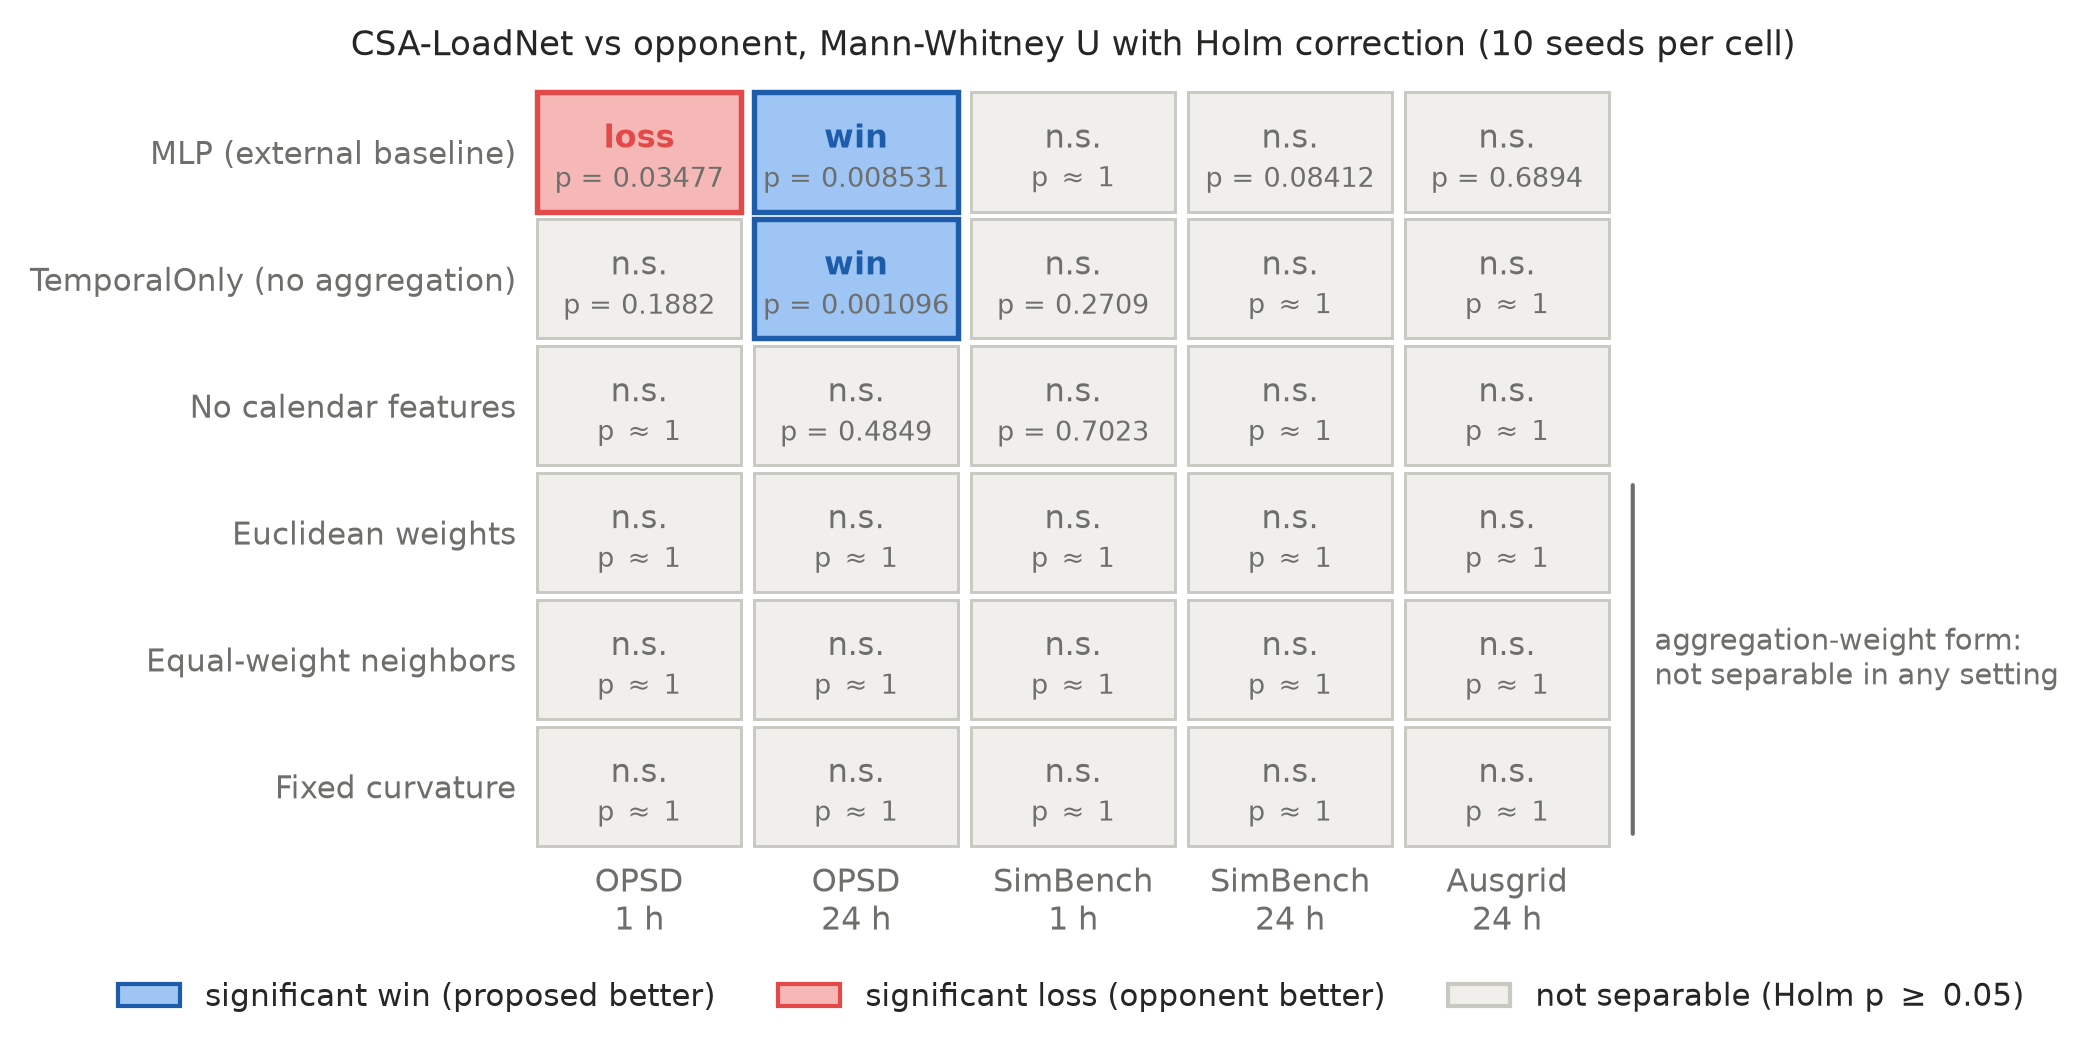
\includegraphics[width=0.94\textwidth]{figures/fig_component.png}
\caption{Historical fixed-split component summary (Mann--Whitney U, Holm-corrected, 10 seeds per cell). Two non-hierarchical fixed-split comparisons are wins--OPSD lead 24 against MLP and against the smaller-head TemporalOnly arm--and OPSD lead 1 contains a loss to MLP. These are not rolling-origin replicates. The corrected hierarchy and its DLinear loss are reported separately in Figures 4--5. The historical weight-form block remains inseparable.}\label{fig:3}
\end{figure*}

The matrix records why stronger controls were needed. At the OPSD fixed split, both the selected external comparison and the smaller-head TemporalOnly comparison separate. At the lead-1 settings, TemporalOnly is nominally worse than the full model but the differences are not significant (OPSD, p = 0.188; SimBench, p = 0.271). The historical aggregation signal is also absent at SimBench lead 24 and Ausgrid (p = 1 in both), with TemporalOnly nominally ahead at SimBench lead 24. No historical weight-form comparison approaches significance. Table 4 supersedes the fixed-split TemporalOnly cell for the aggregation-existence claim.

\subsection{Matched Aggregation and Weighting Controls Do Not Separate}\label{matched-aggregation-and-weighting-controls-do-not-separate}

The matched rolling-origin analysis changes the fixed-split attribution. Cross-series context has a small favorable mean relative to target-self context, but its interval crosses zero and its Holm p is 0.984. The comparison therefore does not establish that aggregation helps under the new estimand. Weighting-form conclusions remain negative:

\begin{itemize}
\tightlist
\item
  \textbf{Poincar\'{e} vs.~Euclidean distance weights:} not separable in the new primary family (mean MAPE difference -0.000009, Holm p = 0.984), consistent with the historical fixed-split nulls.
\item
  \textbf{Poincar\'{e} vs.~uniform neighbor averaging:} not separable in the new family (mean MAPE difference -0.000066, Holm p = 0.984). Learned scores do not demonstrably improve on informative uniform cross-series context.
\item
  \textbf{Learnable vs.~fixed inverse-temperature:} fixed scale is nominally better at seven of eight origins on MAPE and all eight on WAPE. The primary MAPE result does not survive Holm correction (p = 0.0625); secondary WAPE has raw p = 0.0078 but was not multiplicity-adjusted. This is a retained adverse trend, not evidence for the learned scale and not a curvature comparison.
\end{itemize}

The joint conclusion is consequently narrower: neither the existence of cross-series context nor the learned weighting form is established by the matched rolling-origin primary family. Uniform neighbor averaging and target-self context are empirically competitive options, not demonstrated equivalents. The Poincar\'{e} embedding remains an implementation option rather than a supported contribution. The discrepancy with the favorable fixed split illustrates why optimization seeds on one trajectory cannot substitute for temporal replication.

The result is specific to six OPSD series, lead 24, eight quarterly origins, and the frozen budget. Larger pools, sparser cross-correlations, or genuinely tree-structured populations might differ (Section 8). Because no equivalence margin was specified, the unresolved variants are not proven equivalent. The five-seed rolling-origin study also does not retest the MLP comparison, which remains a selected fixed-split result.

\subsection{The Hierarchical Setting: Where the Method Loses}\label{the-hierarchical-setting-where-the-method-loses}

The Ausgrid experiment uses an exact hierarchy built from the 12 selected complete customers: four deterministic postcode-sorted groups each sum three leaves, and the root sums all 12. Figure 4 makes the 17-by-12 summing structure explicit; the identity \(Y=SB\) holds at every hour. Earlier non-exact aggregates are excluded from every result reported here.

\begin{figure*}[t]
\centering
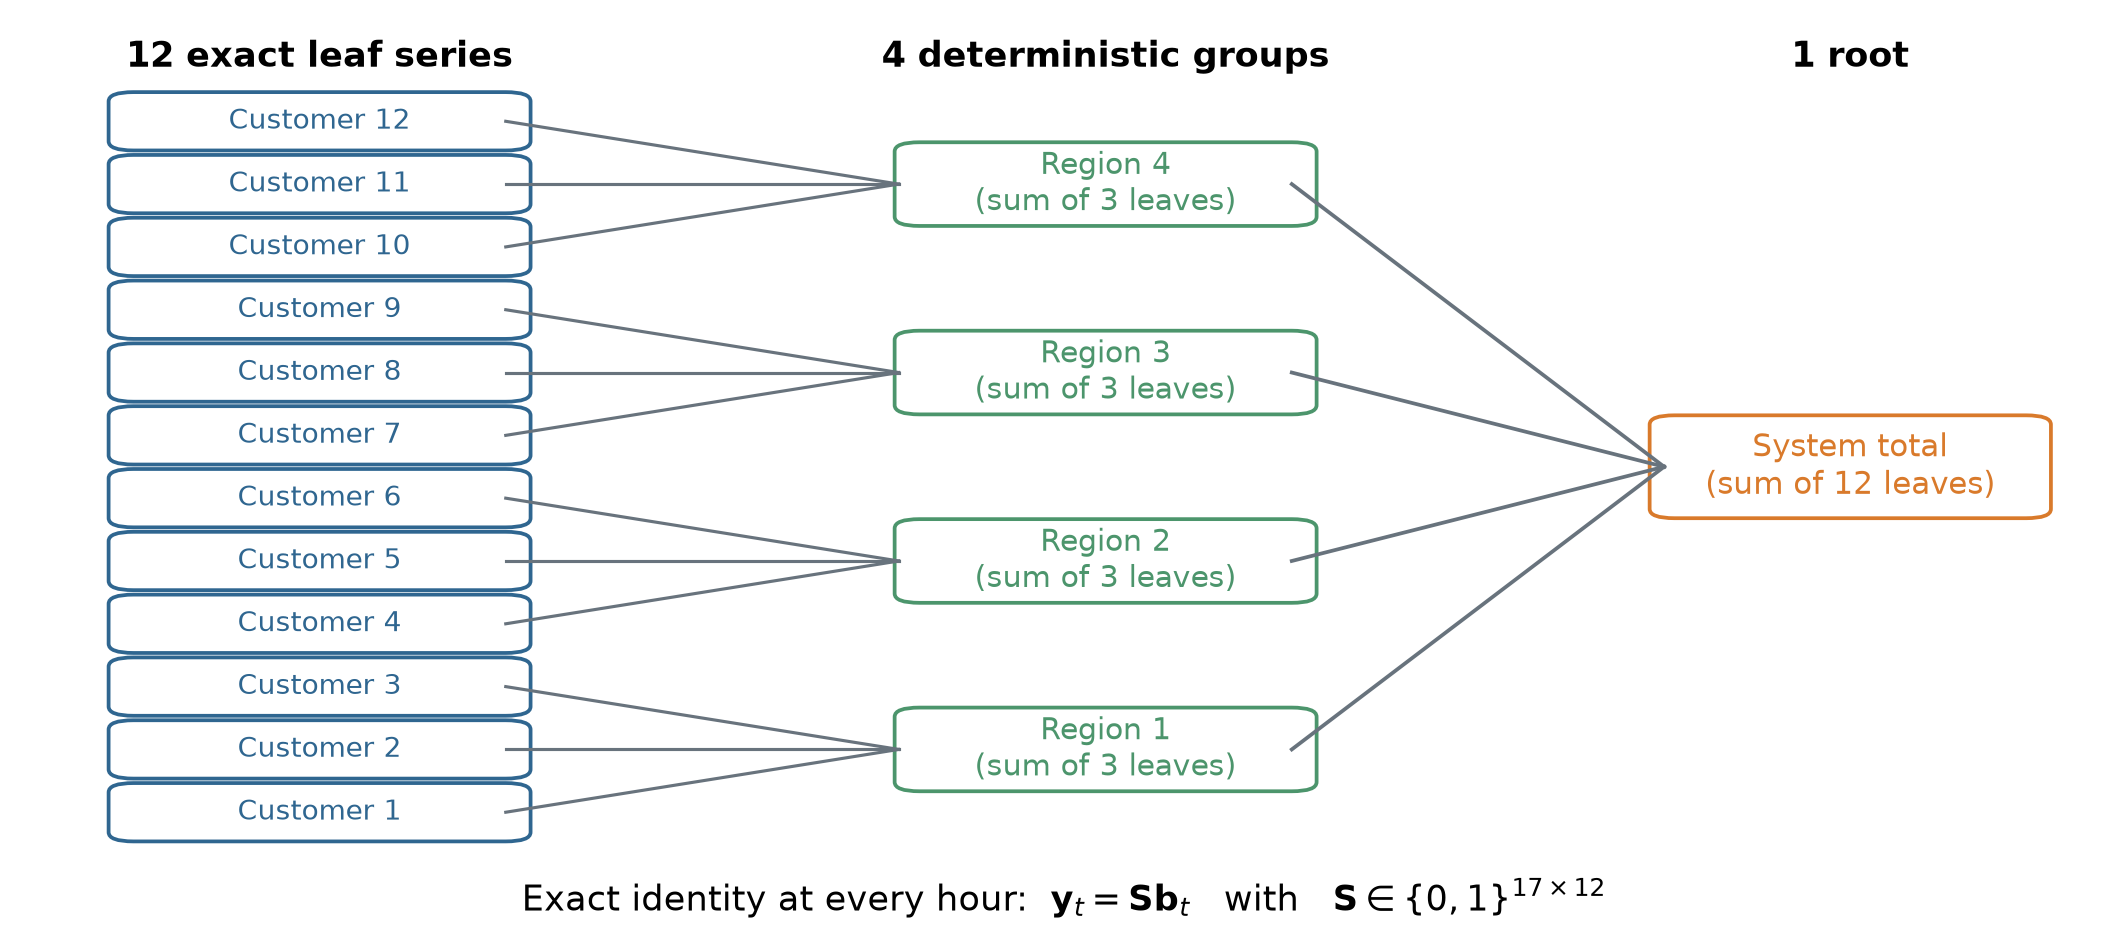
\includegraphics[width=0.94\textwidth]{figures/fig_exact_hierarchy_design.png}
\caption{Corrected Ausgrid hierarchy. The four intermediate series and the system total are deterministic sums of the same 12 leaves used by every forecasting method; no outside customer enters an aggregate.}\label{fig:4}
\end{figure*}

Each trained model first produces an unreconciled matrix \(\hat Y^{\mathrm{base}}\in\mathbb R^{17\times T}\) in the node order 12 leaves, \texttt{region1}--\texttt{region4}, and \texttt{system\_total}. Let \(S\in\{0,1\}^{17\times12}\) be the fixed summing matrix shown in Figure 4. Bottom-up discards the five aggregate-node base forecasts and returns \(\hat Y^{\mathrm{BU}}=S\hat Y^{\mathrm{base}}_{1:12,:}\). Top-down computes leaf proportions \(q_\ell=\sum_{t<b}y_{\ell t}/\sum_{r=1}^{12}\sum_{t<b}y_{rt}\) from the pre-test training segment, allocates the base root forecast as \(q\hat y^{\mathrm{base}}_{17,:}\), and returns \(\hat Y^{\mathrm{TD}}=S(q\hat y^{\mathrm{base}}_{17,:})\). OLS applies the unweighted, covariance-free projection \(P=S(S^{\mathsf T}S)^{-1}S^{\mathsf T}\) independently at every forecasted timestamp: \(\hat Y^{\mathrm{OLS}}=P\hat Y^{\mathrm{base}}\). No post-reconciliation clipping or refitting is implemented. Bottom-up, top-down, and OLS are all exactly coherent by construction; only top-down estimates proportions, and it uses no test targets.

The mean base-forecast coherence violation across the displayed methods is 0.035. Accuracy and coherence are not interchangeable. DLinear with bottom-up reconciliation is best at hierarchy-weighted sMAPE 0.28017, followed by DLinear with OLS at 0.28047. CSA-LoadNet with OLS reaches 0.28949. Under the same OLS transformation, CSA-LoadNet significantly loses to DLinear (Holm \(p=0.000985\)), significantly beats LSTM (\(p=0.000913\)), and is unresolved against MLP, TCN, and PatchTST-lite. The paired CSA-minus-DLinear difference is 0.00902 (pointwise 95\% bootstrap CI {[}0.00606, 0.01215{]}, paired Holm p = 0.0195). The Ausgrid capacity, epoch, and stride asymmetries in Section 5.2 qualify this model-ranking comparison.

\begin{figure*}[t]
\centering
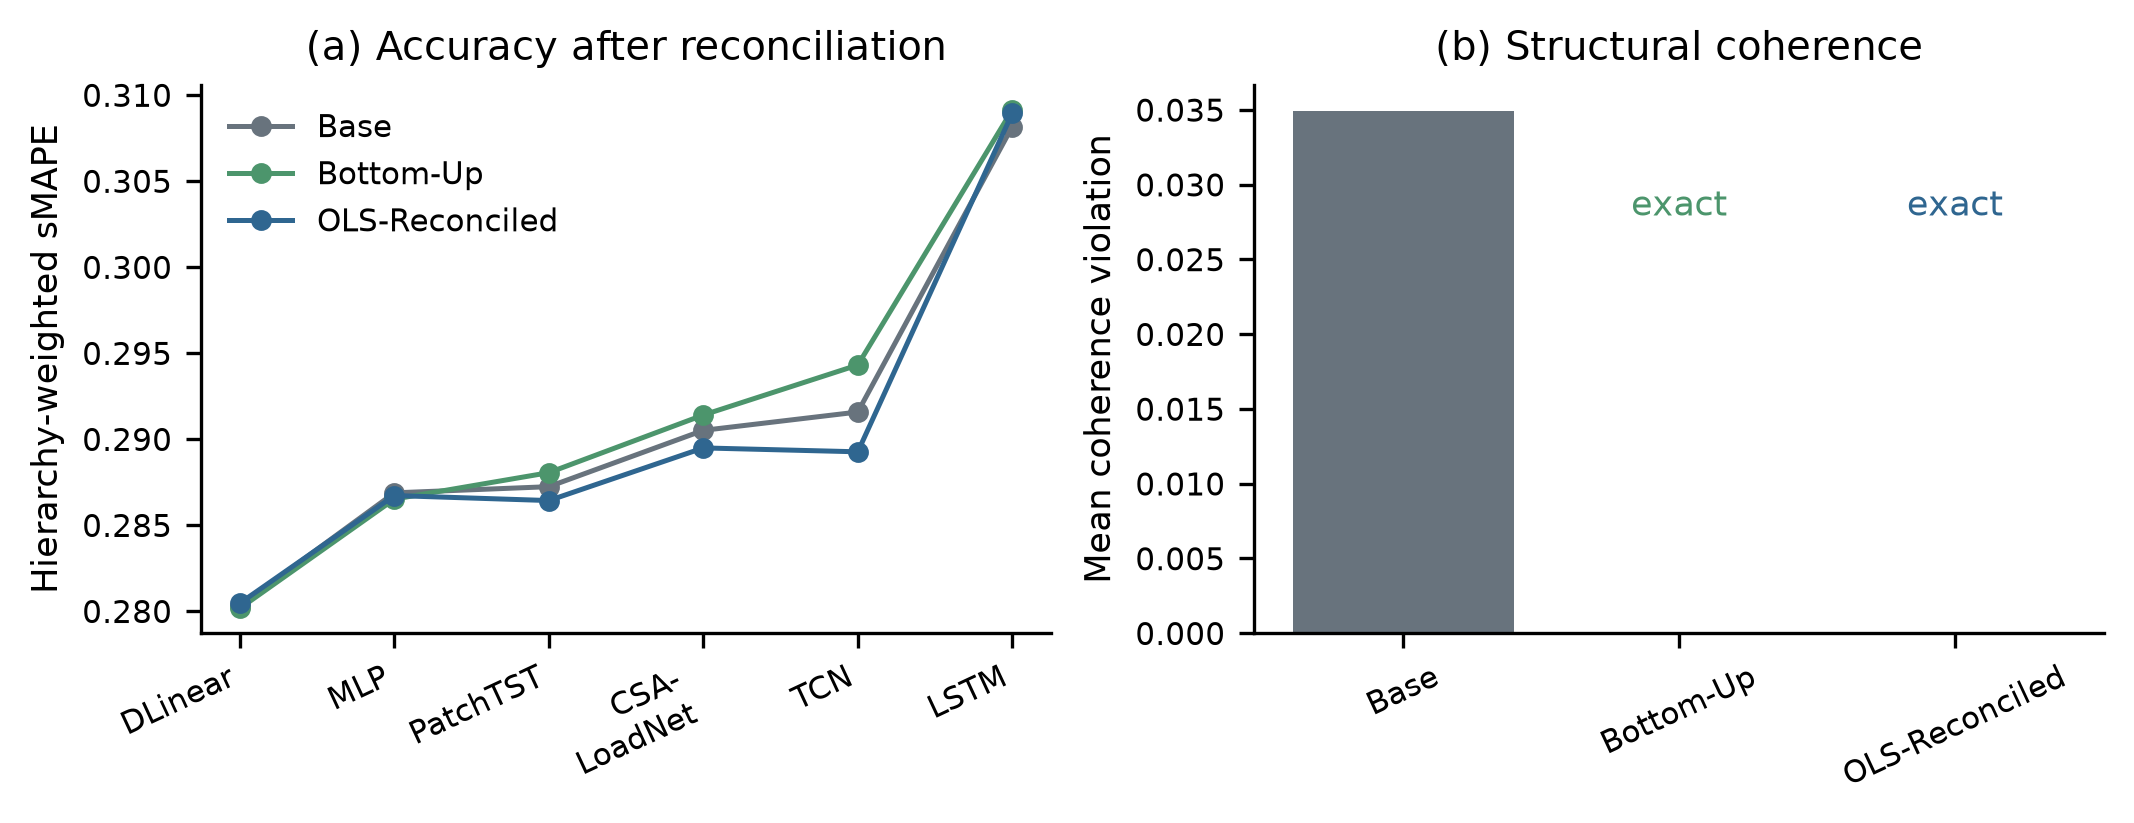
\includegraphics[width=0.94\textwidth]{figures/fig_exact_hierarchy_reconciliation.png}
\caption{(a) Hierarchy-weighted sMAPE under independent, bottom-up, and OLS-reconciled forecasts (ten seeds per model). (b) Mean structural violation. Bottom-up and OLS enforce exact coherence, but DLinear remains more accurate than CSA-LoadNet; reconciliation does not rescue the architectural ranking.}\label{fig:5}
\end{figure*}

The corrected result strengthens the boundary claim rather than the method claim. On the exact customer hierarchy, a strong linear decomposition with deterministic aggregation is better. Together with the new OPSD matched-control null, the evidence does not license reserving CSA-LoadNet for any setting on the basis of an identified aggregation benefit. It does support treating coherence as a separate constraint where accounting identities matter.

\subsection{Short-Horizon and SimBench Boundaries}\label{short-horizon-and-simbench-boundaries}

The remaining cells of Figure 3 complete the boundary map. On OPSD 1 h, the MLP significantly beats CSA-LoadNet (0.010155 versus 0.010689 mean MAPE; primary Holm \(p=0.0348\)). The supplementary paired sensitivity agrees: CSA-minus-MLP MAPE is 0.000534 (pointwise 95\% CI {[}0.000248, 0.000826{]}, paired Holm \(p=0.0469\)). At this lead time, recent target history may dominate the aggregation context. On SimBench, neither horizon separates from the MLP. The proposed mean is only trivially lower at 1 h (0.033349 versus 0.033385 nMAE; \(p=1\)), whereas the MLP mean is lower at 24 h (0.058591 versus 0.060662; \(p=0.084\)). We therefore make no SimBench superiority or parity claim.

Figure 6 expresses the five historical fixed-split comparisons as seed-paired relative error changes. Positive values favor CSA-LoadNet. Only the selected OPSD lead-24 fixed-split comparison combines a positive mean effect with corrected significance. OPSD lead 1 and the corrected Ausgrid hierarchy favor their strongest named comparators; SimBench lead 1 is effectively zero, and SimBench lead 24 trends against the proposed model. The new aggregation-existence decision comes from the origin-level Table 4, not this seed-level display.

\begin{figure*}[t]
\centering
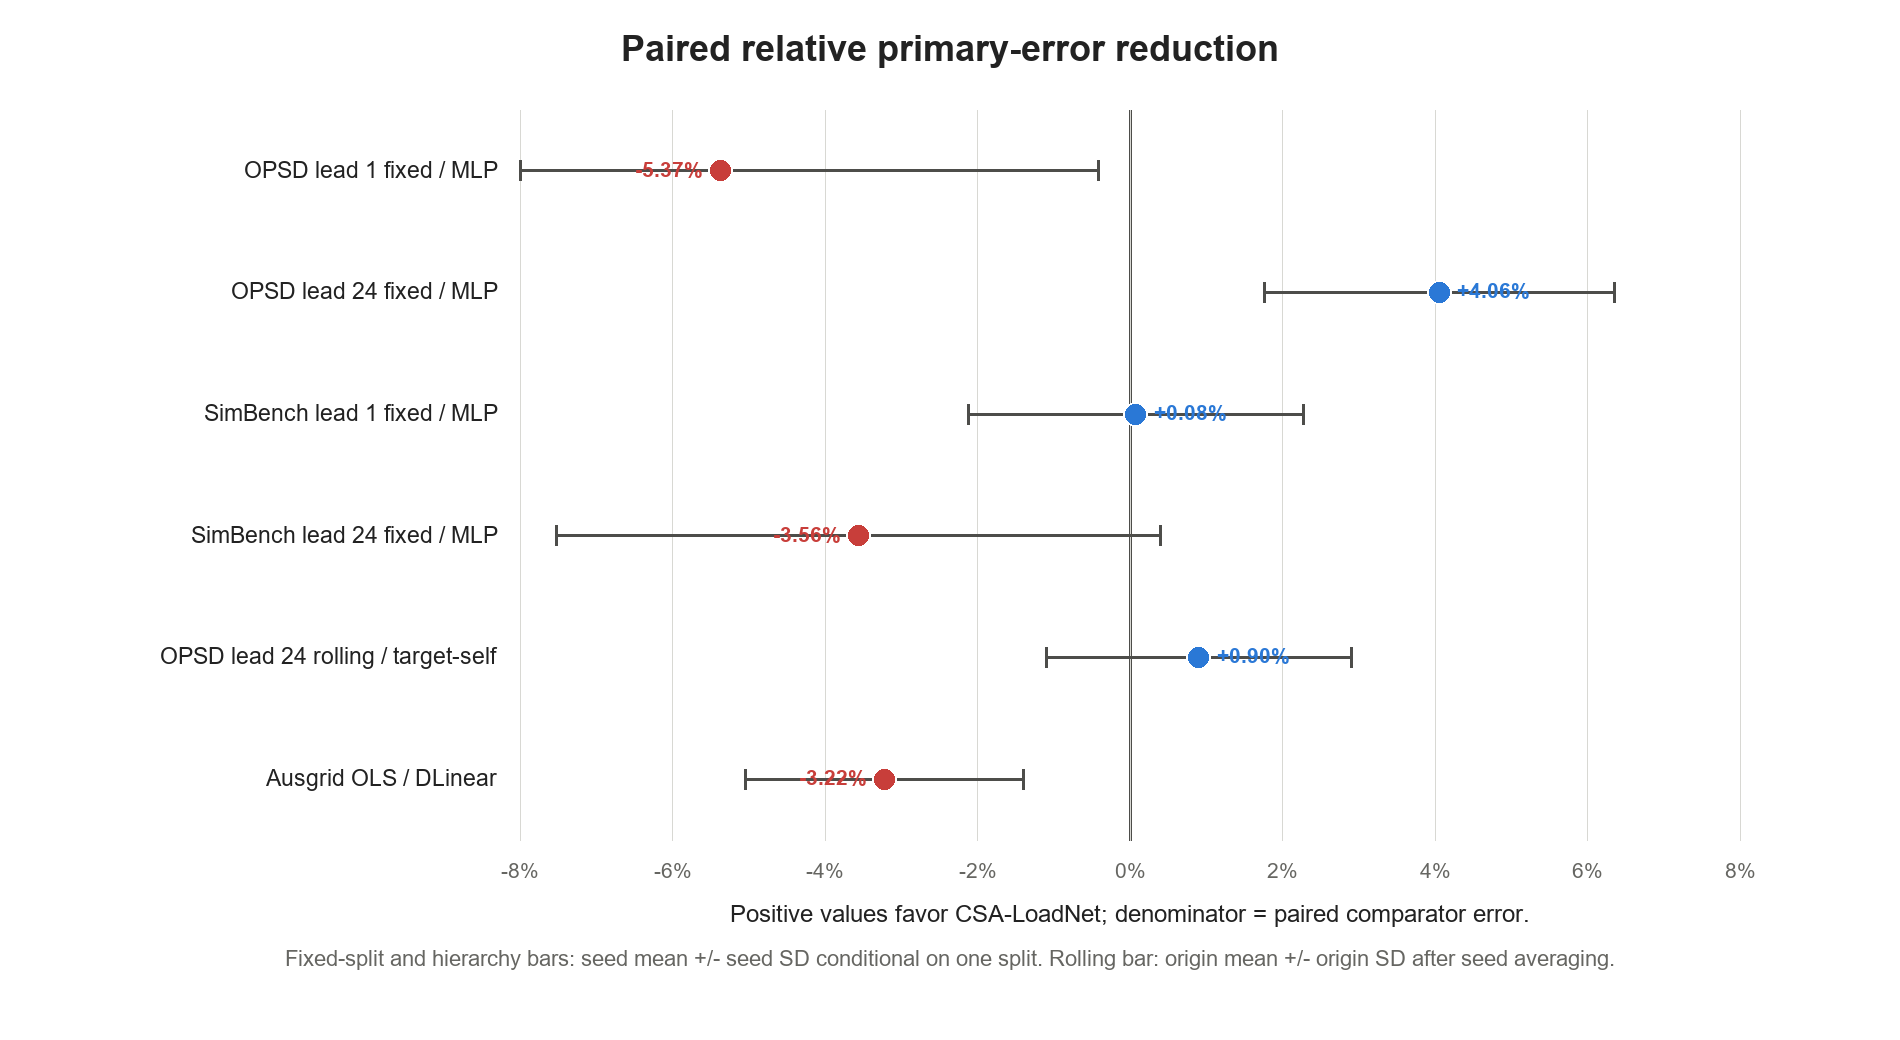
\includegraphics[width=0.94\textwidth]{figures/fig_cross_dataset_effects.png}
\caption{Historical seed-paired relative reduction in each dataset's primary error for CSA-LoadNet against the named comparator. Bars show the mean and error bars show the standard deviation across matched seeds; positive values favor CSA-LoadNet. The historical evidence label \texttt{HyG-LoadFormer (neural)} maps one-to-one to CSA-LoadNet. The matched rolling-origin inference in Table 4 uses a different outer unit and is not encoded by these bars.}\label{fig:6}
\end{figure*}

\subsection{Cross-Setting Rank and Compute Profiles}\label{cross-setting-rank-and-compute-profiles}

Figure 7 preserves the historical fixed-split rank profile. Every historically available model is ranked by the prespecified primary metric in each of the five dataset--horizon settings; the Ausgrid column uses the exact hierarchy under common OLS reconciliation. CSA-LoadNet ranks in the middle of the OPSD lead-1 field, first on the OPSD lead-24 fixed split, near the front but unresolved against several methods on SimBench, and below DLinear on Ausgrid. The new matched controls are not included in this historical figure; their origin-level ranks appear in Table 4. Missing cells are not imputed, and no cross-dataset average rank is formed because the metrics have different meanings.

\begin{figure*}[t]
\centering
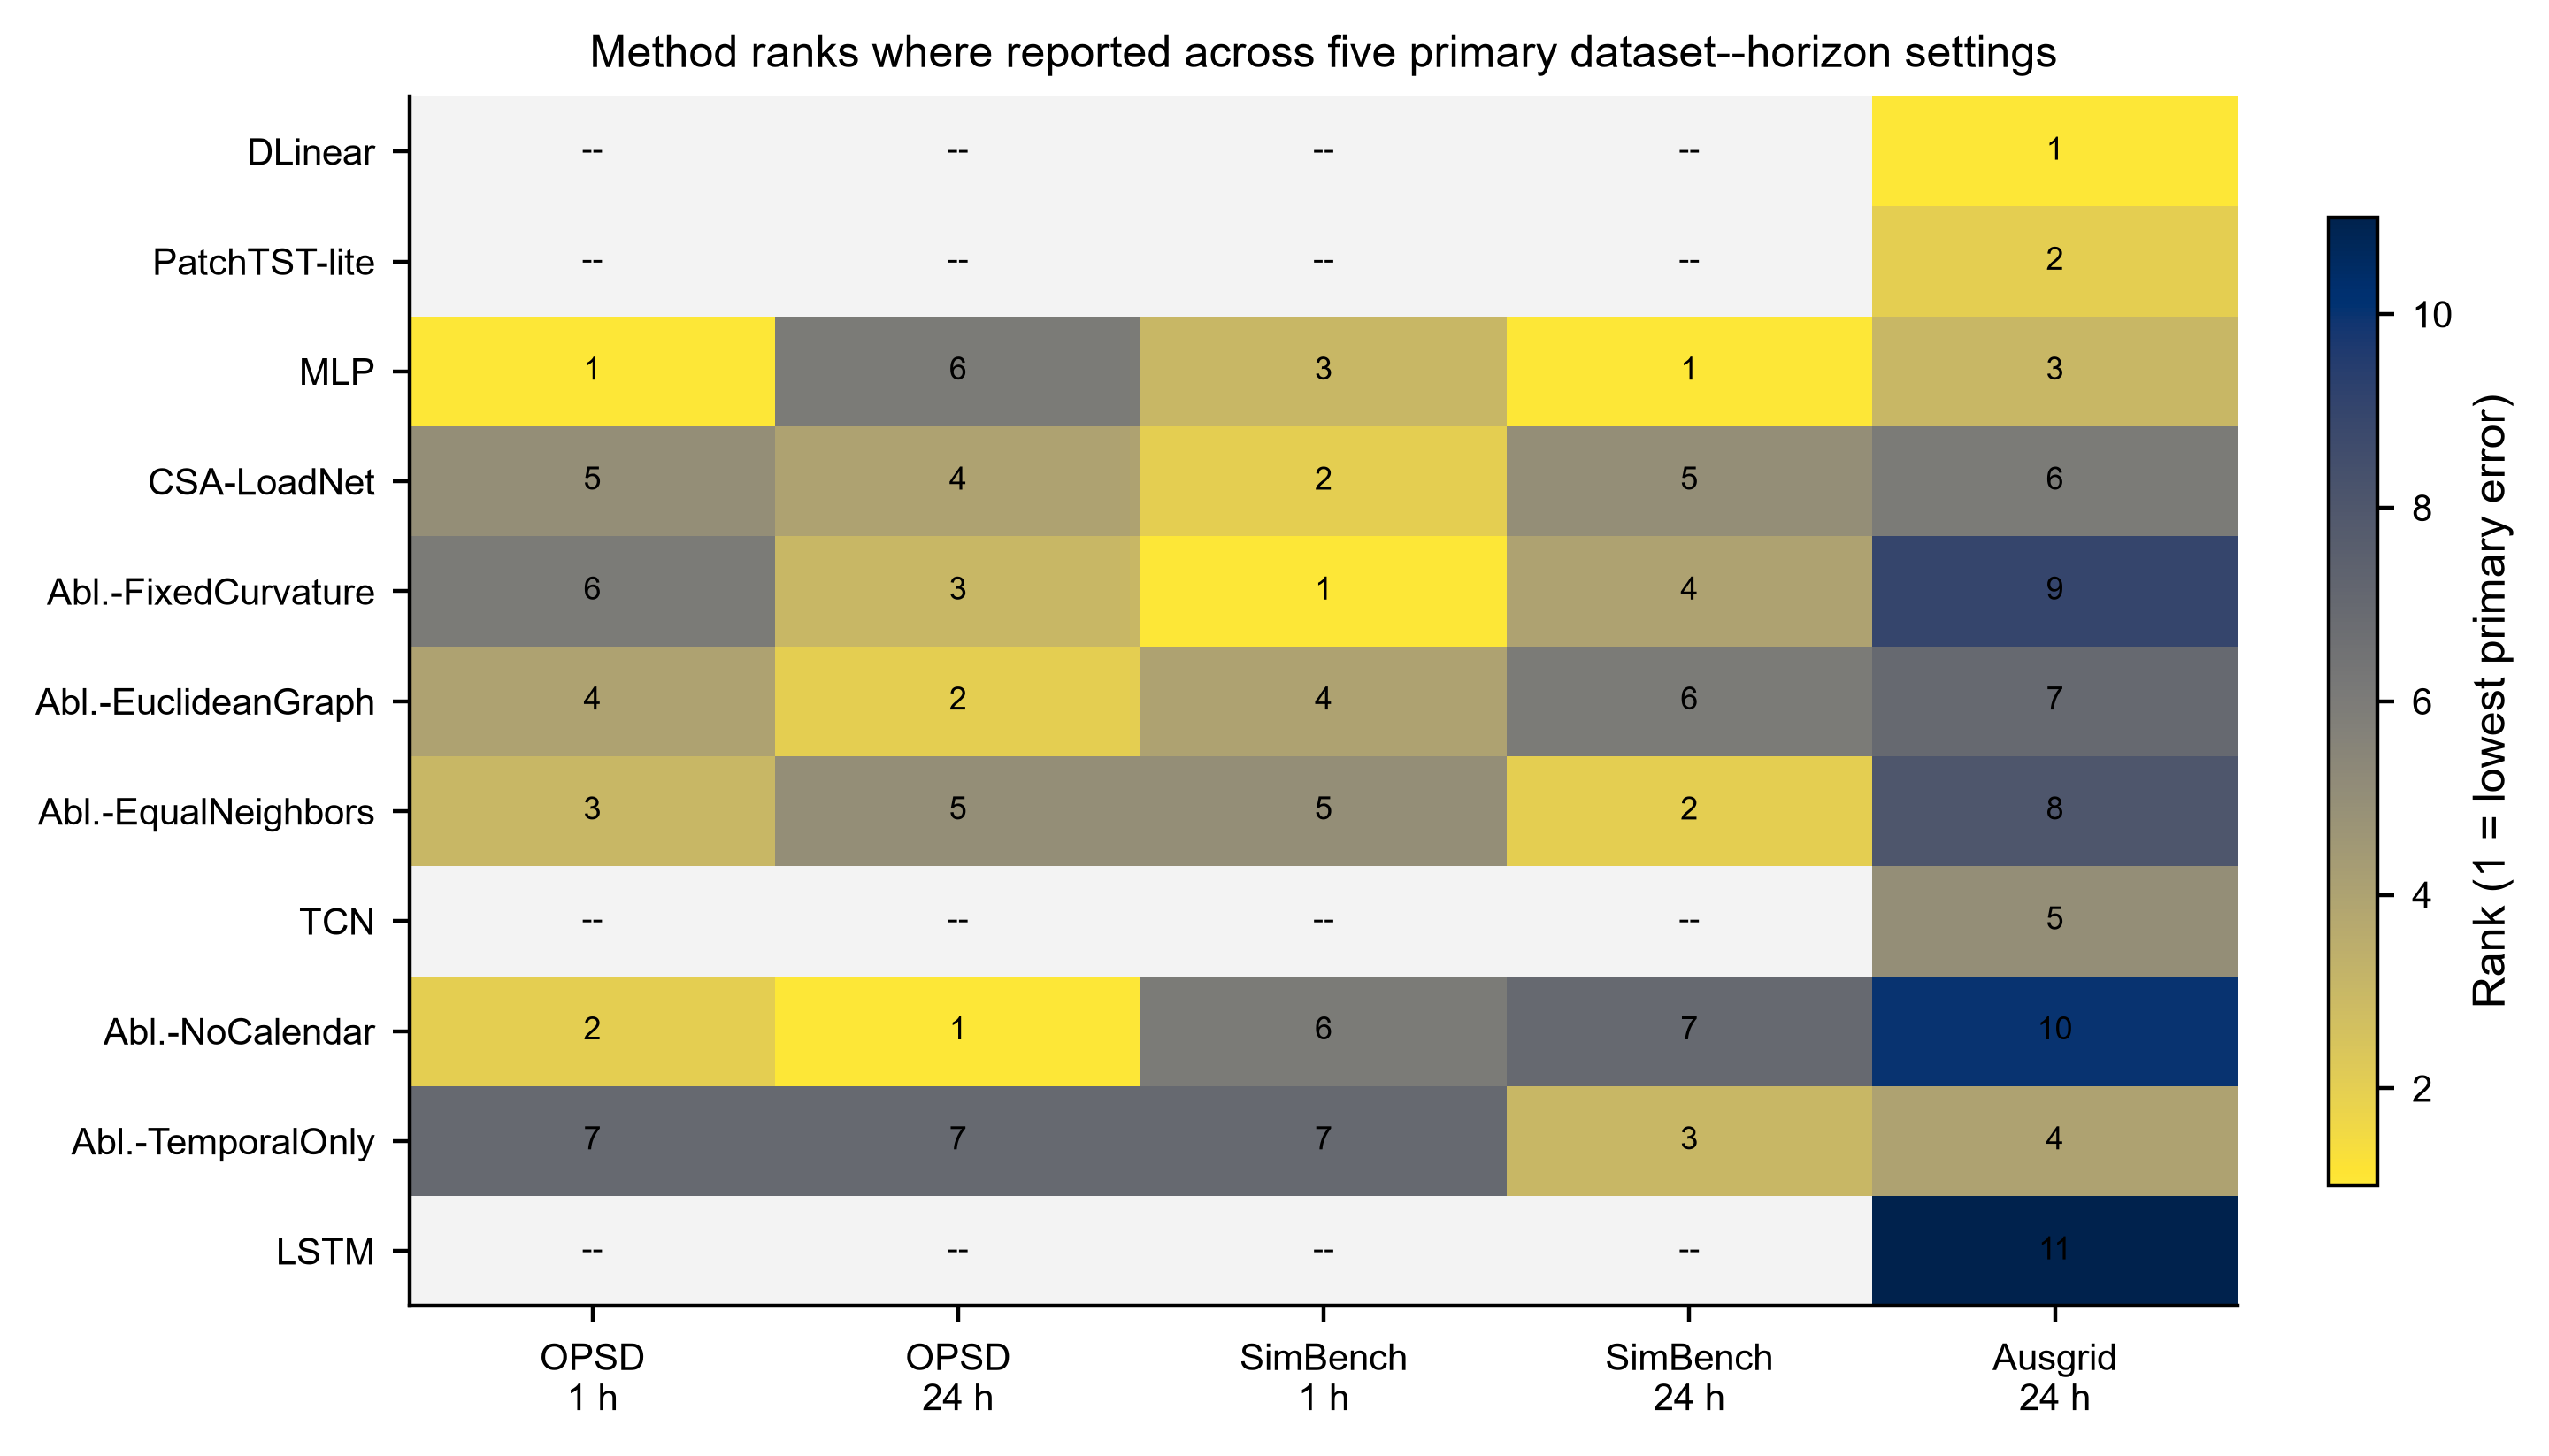
\includegraphics[width=0.94\textwidth]{figures/fig_cross_setting_ranks.png}
\caption{Ranks by dataset-specific primary error. Rank 1 is the lowest mean error within a column. Dashes mark methods absent from an experiment. Non-hierarchical cells use the ten-seed OPSD and SimBench leaderboards; the Ausgrid column uses the exact hierarchy with OLS reconciliation.}\label{fig:7}
\end{figure*}

The run-time profile in Figure 8 supplies the computational counterpart. The same compact architecture is inexpensive on OPSD and SimBench and slower on the 17-series Ausgrid hierarchy. The y-axis intentionally retains each dataset's primary metric, so vertical locations must not be compared across datasets; the panel asks whether a reported accuracy cell is accompanied by an exceptional computational burden, not whether the error scales are interchangeable.

\begin{figure*}[t]
\centering
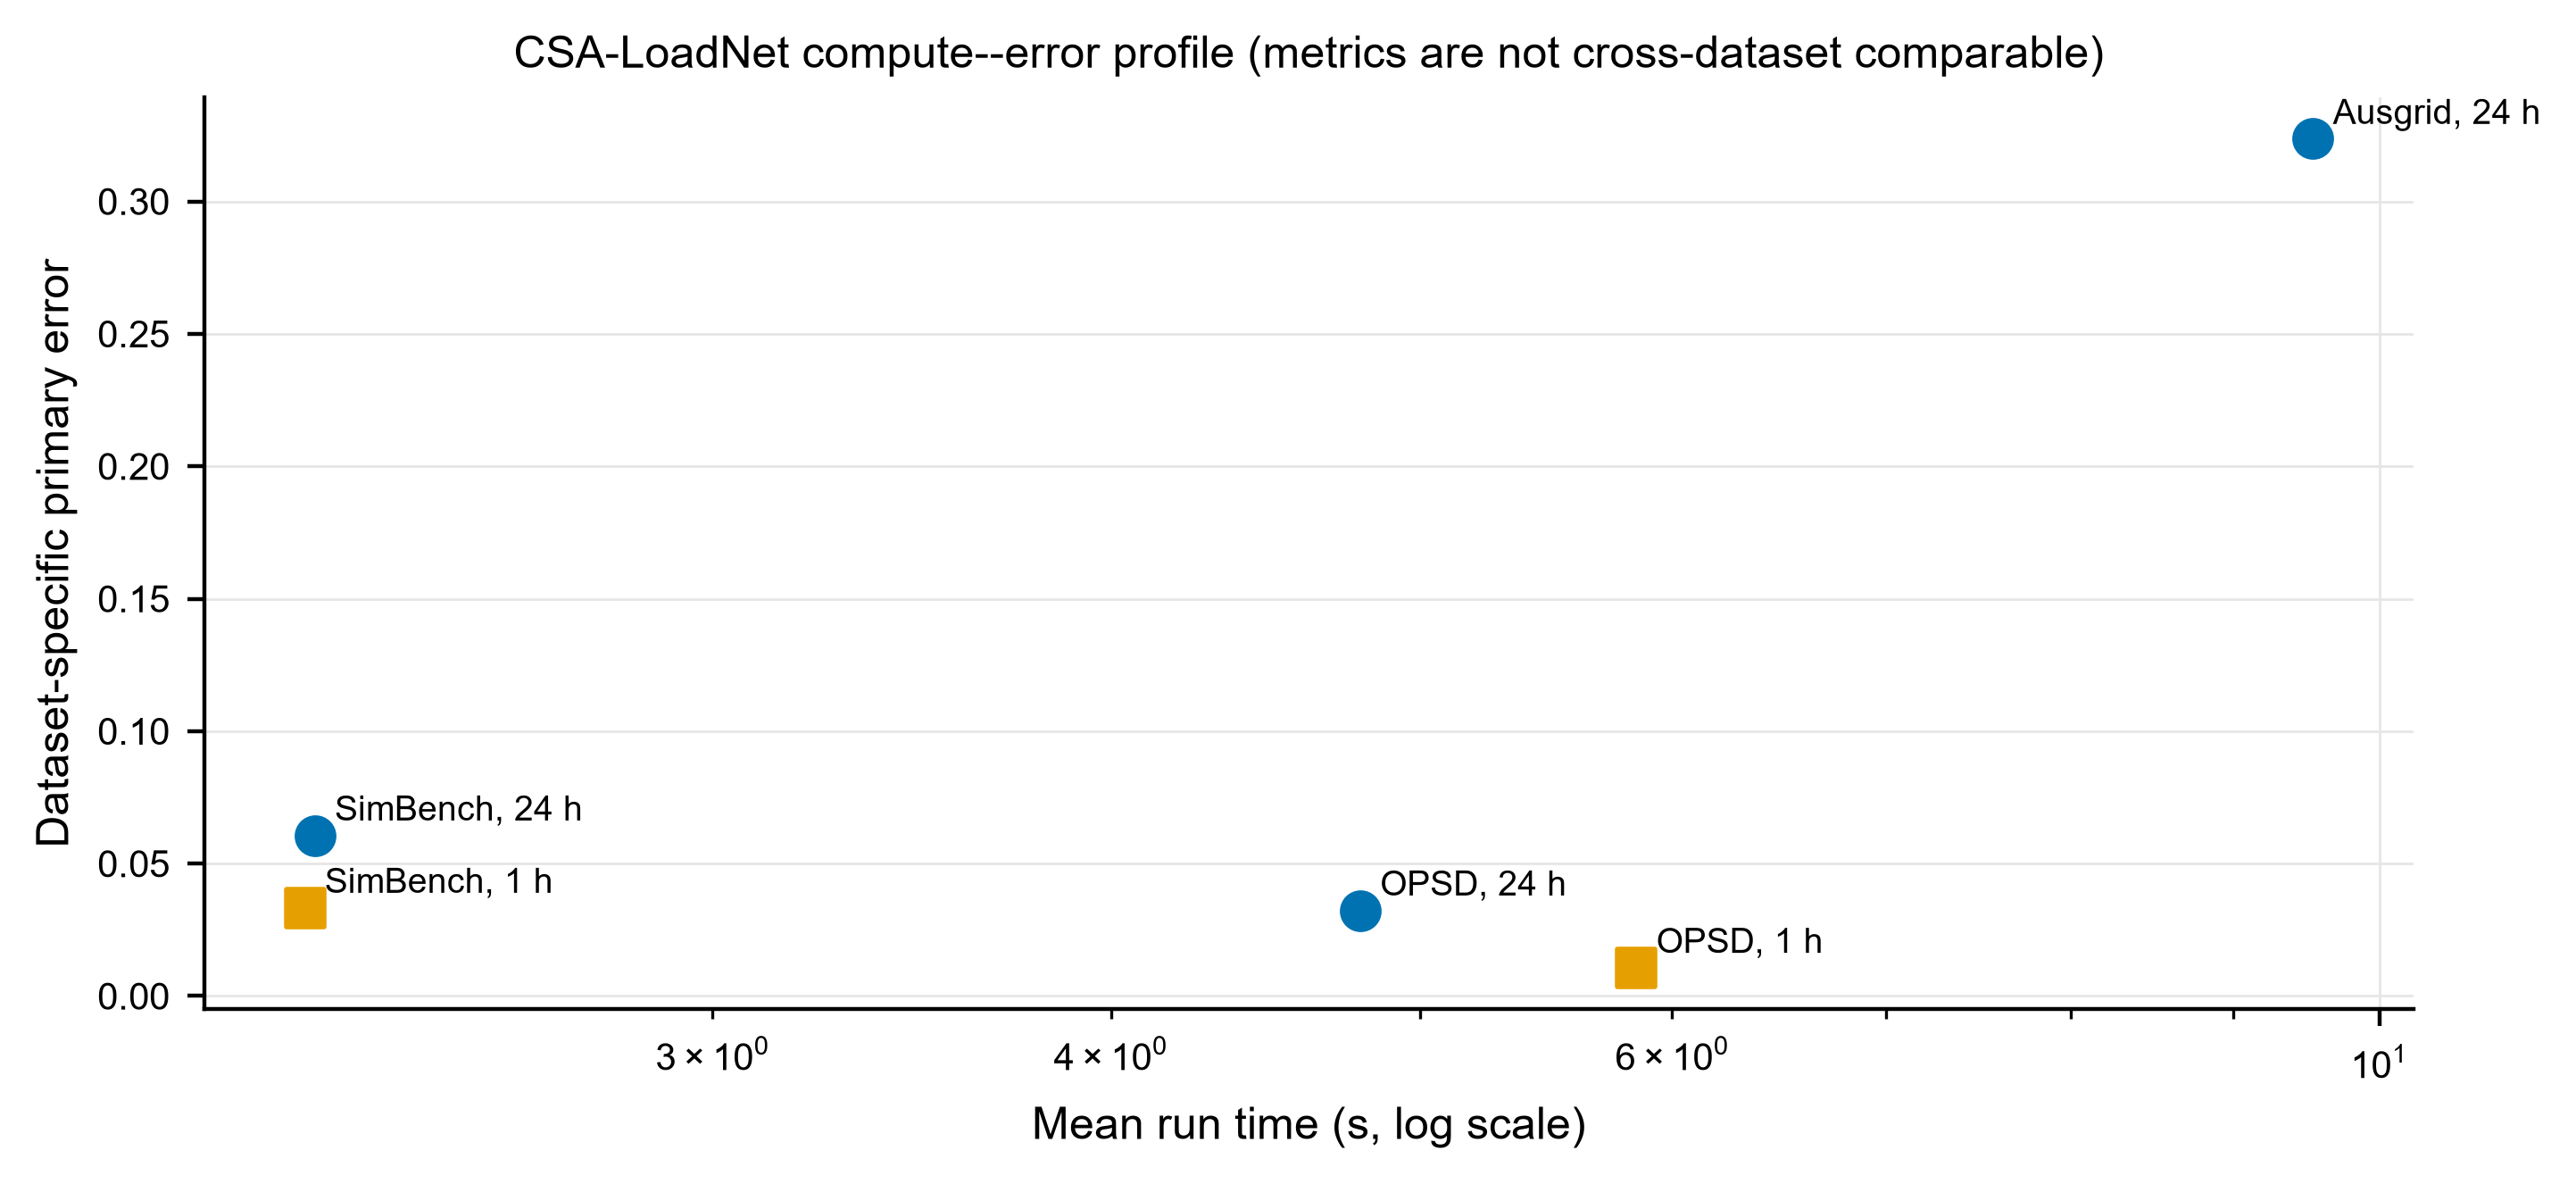
\includegraphics[width=0.94\textwidth]{figures/fig_compute_error_profile.png}
\caption{Mean wall-clock time and dataset-specific primary error for CSA-LoadNet at each evaluated horizon. The x-axis is logarithmic. Timings are interpreted within dataset and execution environment, not across CPU and GPU blocks.}\label{fig:8}
\end{figure*}

\begin{table*}[t]
\centering
\footnotesize
\setlength{\tabcolsep}{3pt}
\caption{Stability summary across the complete primary-metric comparisons. "Supported" requires Holm-adjusted (p<0.05); a nominal mean ordering without corrected separation is not counted.}\label{tab:6}
\begin{tabularx}{\textwidth}{@{}>{\raggedright\arraybackslash}X >{\raggedright\arraybackslash}X >{\raggedright\arraybackslash}X >{\raggedright\arraybackslash}X@{}}
\toprule
Setting & Proposed mean position & Corrected decision against strongest named baseline & Interpretation \\
\midrule
OPSD, 1 h & Behind MLP & Significant loss & Short-horizon boundary \\
OPSD, lead 24 fixed split & Ahead of selected MLP & Significant win & Historical selected-comparator result \\
OPSD, lead 24 rolling origins & Ahead of matched target-self control by 0.69\% & Not separable & Aggregation-existence claim not confirmed \\
SimBench, 1 h & Approximately tied & Not separable & No superiority claim \\
SimBench, 24 h & Behind MLP & Not separable & Adverse nominal trend \\
Ausgrid, 24 h & Behind DLinear under OLS & Significant loss & Coherence achieved; no accuracy-superiority claim \\
\bottomrule
\end{tabularx}
\end{table*}

The table and rank profile separate two levels of evidence. The selected MLP comparison remains favorable on one fixed split, but cross-series aggregation does not separate from the capacity-matched target-self control over eight rolling origins. The tested attention parameterizations likewise remain unresolved. The evidence supports a component-evaluation result, not an aggregation-performance claim.

\begin{center}\rule{0.5\linewidth}{0.5pt}\end{center}

\section{Discussion}\label{discussion}

\subsection{Aggregation, Weighting, and Hierarchical Coherence}\label{aggregation-weighting-and-hierarchical-coherence}

The historical ten-seed fixed split favors CSA-LoadNet over the smaller-head TemporalOnly arm and the selected MLP. The new matched analysis does not reproduce the aggregation separation: target-self context is only 0.69\% worse in mean MAPE and the Holm-adjusted p is 0.984. Learned Poincar\'{e}, uniform, and Euclidean cross-series weighting also do not separate. The fixed-scale arm is nominally best, including lower WAPE at every origin, but its primary MAPE p becomes 0.0625 after correction. The preliminary architecture screen and the single favorable fixed split therefore cannot carry a confirmatory aggregation claim.

The exact Ausgrid experiment answers a different question. It constructs all four regional aggregates and the root from the same 12 leaves and applies common reconciliation transformations to every method. Bottom-up and OLS reconciliation remove structural violations, yet DLinear remains more accurate than CSA-LoadNet. Coherence is therefore a constraint that can be enforced after forecasting; it is not evidence that the underlying forecaster is accurate.

Taken together, the experiments locate uncertainty rather than a benefit. Pool context is not separated from a matched target-only context over the evaluated OPSD origins, and additional weighting complexity is unsupported. The shared encoder outperforms the parameter-matched independent arm, but that control changes hidden widths and arithmetic, so sharing itself remains unresolved. Independently repeated weather years and a compute-matched independent encoder would be needed to test either mechanism more cleanly.

\subsection{Horizon Interpretation Remains Unresolved}\label{horizon-interpretation-remains-unresolved}

The historical horizon asymmetry admits a hypothesis but not a demonstrated mechanism. At lead 1, each country's own recent observations may contain most recoverable information; at lead 24, synchronized daily and weekly shapes could supply useful context. However, the lead-24 matched rolling-origin comparison does not establish a context benefit, and the new namespace does not rerun lead 1. Because no weather variables or mechanism intervention links the series, the study does not claim why errors differ by horizon.

\subsection{Implications for the Cross-Series Forecasting Literature}\label{implications-for-the-cross-series-forecasting-literature}

Our results neither reject cross-series modeling nor support an aggregation or weighting advantage. The historical smaller-head TemporalOnly contrast suggested a 6.5\% fixed-split difference, whereas the matched rolling-origin contrast shrinks to a 0.69\% mean MAPE difference and is unresolved. No primary-family weighting-form difference is established; equivalence within a prespecified tolerance was not tested. This discrepancy shows why mechanism claims require both matched component controls and temporal replication. The new OPSD control study and the earlier exact-hierarchy rerun used a single RTX 3090; the historical OPSD and SimBench decision sets used CPU execution.

\begin{center}\rule{0.5\linewidth}{0.5pt}\end{center}

\section{Limitations}\label{limitations}

\begin{enumerate}
\def\labelenumi{\arabic{enumi}.}
\tightlist
\item
  \textbf{No aggregation superiority claim survives the matched temporal analysis.} The historical fixed split favors CSA-LoadNet over the selected MLP and smaller-head TemporalOnly arms, but the matched target-self contrast over eight rolling origins is unresolved (MAPE Holm \(p=0.984\); secondary WAPE raw \(p=0.227\)). The experiment predicts one scalar at lead 24 and does not score a 24-point next-day trajectory. The historical OPSD lead-1 comparison favors MLP, and neither SimBench lead separates from MLP.
\item
  \textbf{The method does not transfer to the exact customer/region/system hierarchy as implemented.} Under common OLS reconciliation, CSA-LoadNet significantly loses to DLinear (Holm \(p<0.001\)), while its contrasts against MLP, TCN, and PatchTST-lite remain unresolved under the primary family. Bottom-up, top-down, and OLS reconciliation satisfy the accounting identities, but coherence does not establish forecaster accuracy. MinT with covariance shrinkage and end-to-end coherence-constrained training remain untested.
\item
  \textbf{The weight-form inseparability is a bounded negative.} Learned Poincar\'{e} weighting does not separate from uniform or Euclidean context in the new primary family, consistent with historical nulls across pools of 6, 8, and 17 series. Fixed scale is nominally better in the new study (MAPE Holm \(p=0.0625\); secondary WAPE raw \(p=0.0078\)), so the data do not favor learned scaling. No equivalence margin was specified.
\item
  \textbf{Only the new shared-encoder component arms are parameter- and head-matched.} Historical external-model counts range from 338 to 70,597 and epoch budgets differ. On Ausgrid, CSA variants use stride 6 while external baselines use stride 3, and the run CSV misrecords the baseline exposure. The new independent-encoder arm matches total parameters but changes hidden widths and uses substantially less encoder arithmetic. Neither the historical rankings nor the shared-encoder contrast is a fully capacity-and-compute-controlled causal comparison.
\item
  \textbf{Ausgrid structural selection sees the full record.} The completeness filter and top-energy leaf ranking use all three years before the chronological split. This does not train model parameters on test targets, but it is not a train-only selection design and may favor continuous, high-consumption customers. Only one deterministic grouping is tested.
\item
  \textbf{Timestamp and missingness handling are limited.} OPSD is kept in UTC, whereas SimBench and constructed Ausgrid labels have no represented timezone and receive no daylight-saving adjustment. Sequence-phase covariates come from row indices rather than parsed timestamps. The new OPSD run records 43 discarded source rows before reaching 35,000 retained rows, so a 24-position lead is not always 24 elapsed UTC hours around gaps. SimBench discard counts remain unavailable, and Ausgrid blank half-hours are set to zero. Sensitivity to these choices is untested.
\item
  \textbf{Temporal replication remains within one observed record.} The eight quarterly origins span 2017--2018, use adjacent portions of the same six country series, and are not independent weather-year or system replications. The exact sign-flip test assumes exchangeable origin differences; quarterly spacing reduces test-block overlap but does not establish independence. MLP selection still used the historical fixed test trajectory and was not rerun in the new confirmatory family.
\item
  \textbf{No exogenous weather or operational covariates are used.} All models forecast from load history and four row-index phase features. Weather-aware extensions, holidays, localized civil time, dispatch consequences, and deployment remain untested.
\item
  \textbf{The new namespace has not been independently rerun.} Its hashes, environment, frozen configuration, raw rows, origin tables, and analysis code are retained, but reproducibility status remains \texttt{UNVERIFIED} until a separate immutable rerun is compared.
\end{enumerate}

\begin{center}\rule{0.5\linewidth}{0.5pt}\end{center}

\section{Conclusions}\label{conclusions}

This study tests which components of a cross-series attention forecaster remain supported after capacity matching and temporal replication. The earlier OPSD fixed split favors CSA-LoadNet over a selected MLP and a smaller-head TemporalOnly arm, but the new eight-origin analysis does not separate it from a matched target-self context: mean MAPE is 0.036640 versus 0.036894 (Holm \(p=0.984\)), and mean WAPE is 0.036775 versus 0.037109 (raw \(p=0.227\)). The fixed-split aggregation attribution therefore does not replicate under the new estimand.

The form of the aggregation weights is likewise unsupported as a differentiator. Learned Poincar\'{e} weights do not separate from uniform or Euclidean context after correction, and fixed scaling is nominally better rather than worse. The shared encoder beats the parameter-matched independent arm, but width allocation and arithmetic differ, precluding a sharing claim. Historical OPSD lead-1, SimBench, and exact-hierarchy Ausgrid findings remain adverse or unresolved; reconciliation supplies coherence, not accuracy superiority. The resulting contribution is a matched null result, an empirical limit on weighting complexity, and a separation between forecast accuracy and structural coherence.

\begin{center}\rule{0.5\linewidth}{0.5pt}\end{center}

\section*{Author Contributions}

{[}AUTHOR INPUT REQUIRED: assign the CRediT roles to Jieyun Zheng, Linyao Zhang, Zhanghuang Zhang, Zhuolin Chen, and Ying Shi, and obtain approval from every author.{]} All authors have read and agreed to the published version of the manuscript.

\section*{Funding}

{[}AUTHOR INPUT REQUIRED: insert the verified funder, grant number, and APC funder, or state ``This research received no external funding.''{]}

\section*{Institutional Review Board Statement}

Not applicable.

\section*{Informed Consent Statement}

Not applicable.

\section*{Data Availability Statement}

All datasets used in this study are public: the Open Power System Data 60 min package (https://open-power-system-data.org) {[}29{]}, SimBench load profiles (https://simbench.de) {[}30{]}, and Ausgrid solar-home electricity data (https://www.ausgrid.com.au) {[}24{]}. The supplementary package contains the CSA-LoadNet implementation and configurations; 280 historical non-hierarchical decision-set records; 440 exact-hierarchy model--reconciliation records; and the new immutable namespace with 240 method--origin--seed rows, 6,750 forecast-day audit rows, origin-level inference, hashes, and validation report. These assets are available from the corresponding author. A persistent public archive can be supplied before publication, subject to source-data terms. Archived historical CSV files use the full-configuration label \texttt{HyG-LoadFormer\ (neural)}, whose one-to-one mapping to CSA-LoadNet is documented in the evidence README.

\section*{Acknowledgments}

During the preparation of this manuscript, the authors used Claude (Anthropic) for language drafting and editing and for assistance in preparing analysis and figure-generation code. All experimental designs, data processing steps, numerical results, statistical analyses, and conclusions were specified, executed, and verified by the authors. The authors reviewed and revised all assisted content and take full responsibility for the publication.

\section*{Conflicts of Interest}

The authors declare no conflicts of interest.

\begin{center}\rule{0.5\linewidth}{0.5pt}\end{center}

\begin{thebibliography}{99}
\bibitem{ref1} Li, J.; Li, J.; Li, J.; Zhang, G. Bayesian-Optimized GCN-BiLSTM-Adaboost Model for Power-Load Forecasting. \emph{Electronics} \textbf{2025}, \emph{14}(16), 3332. \url{https://doi.org/10.3390/electronics14163332}
\bibitem{ref2} Zhou, H.; Ai, Q.; Li, R. Short-Term Multi-Energy Load Forecasting Method Based on Transformer Spatio-Temporal Graph Neural Network. \emph{Energies} \textbf{2025}, \emph{18}(17), 4466. \url{https://doi.org/10.3390/en18174466}
\bibitem{ref3} Wu, M.; Feng, W.; Li, X.; Liu, Y.; Cao, C. Short-Term Power Load Forecasting Using an Improved Model Integrating GCN and Transformer. \emph{Applied Sciences} \textbf{2025}, \emph{15}(13), 7003. \url{https://doi.org/10.3390/app15137003}
\bibitem{ref4} Zhang, J.; Yu, B.; Lai, H.; Liu, L.; Zhou, J.; Lou, F.; Ni, Y.; Peng, Y.; Yu, Z. LoadSeer: Exploiting Tensor Graph Convolutional Network for Power Load Forecasting With Spatio-Temporal Characteristics. \emph{IEEE Access} \textbf{2024}, \emph{12}, 190337--190346. \url{https://doi.org/10.1109/ACCESS.2024.3514174}
\bibitem{ref5} Zeng, A.; Chen, M.; Zhang, L.; Xu, Q. Are Transformers Effective for Time Series Forecasting? \emph{Proceedings of the AAAI Conference on Artificial Intelligence} \textbf{2023}, \emph{37}(9), 11121--11128. \url{https://doi.org/10.1609/aaai.v37i9.26317}
\bibitem{ref6} Makridakis, S.; Spiliotis, E.; Assimakopoulos, V. Statistical and Machine Learning forecasting methods: Concerns and ways forward. \emph{PLOS ONE} \textbf{2018}, \emph{13}(3), e0194889. \url{https://doi.org/10.1371/journal.pone.0194889}
\bibitem{ref7} Makridakis, S.; Spiliotis, E.; Assimakopoulos, V. The M4 Competition: 100,000 time series and 61 forecasting methods. \emph{International Journal of Forecasting} \textbf{2020}, \emph{36}(1), 54--74. \url{https://doi.org/10.1016/j.ijforecast.2019.04.014}
\bibitem{ref8} Hewamalage, H.; Ackermann, K.; Bergmeir, C. Forecast evaluation for data scientists: common pitfalls and best practices. \emph{Data Mining and Knowledge Discovery} \textbf{2023}, \emph{37}(2), 788--832. \url{https://doi.org/10.1007/s10618-022-00894-5}
\bibitem{ref9} Hochreiter, S.; Schmidhuber, J. Long Short-Term Memory. \emph{Neural Computation} \textbf{1997}, \emph{9}(8), 1735--1780. \url{https://doi.org/10.1162/neco.1997.9.8.1735}
\bibitem{ref10} Kong, W.; Dong, Z.Y.; Jia, Y.; Hill, D.J.; Xu, Y.; Zhang, Y. Short-Term Residential Load Forecasting Based on LSTM Recurrent Neural Network. \emph{IEEE Transactions on Smart Grid} \textbf{2019}, \emph{10}(1), 841--851. \url{https://doi.org/10.1109/TSG.2017.2753802}
\bibitem{ref11} Salinas, D.; Flunkert, V.; Gasthaus, J.; Januschowski, T. DeepAR: Probabilistic forecasting with autoregressive recurrent networks. \emph{International Journal of Forecasting} \textbf{2020}, \emph{36}(3), 1181--1191. \url{https://doi.org/10.1016/j.ijforecast.2019.07.001}
\bibitem{ref12} Lara-Ben\'{\i}tez, P.; Carranza-Garc\'{\i}a, M.; Luna-Romera, J.M.; Riquelme, J.C. Temporal Convolutional Networks Applied to Energy-Related Time Series Forecasting. \emph{Applied Sciences} \textbf{2020}, \emph{10}(7), 2322. \url{https://doi.org/10.3390/app10072322}
\bibitem{ref13} Lim, B.; Ar\i{}k, S.\"{O}.; Loeff, N.; Pfister, T. Temporal Fusion Transformers for interpretable multi-horizon time series forecasting. \emph{International Journal of Forecasting} \textbf{2021}, \emph{37}(4), 1748--1764. \url{https://doi.org/10.1016/j.ijforecast.2021.03.012}
\bibitem{ref14} Zhou, H.; Zhang, S.; Peng, J.; Zhang, S.; Li, J.; Xiong, H.; Zhang, W. Informer: Beyond Efficient Transformer for Long Sequence Time-Series Forecasting. \emph{Proceedings of the AAAI Conference on Artificial Intelligence} \textbf{2021}, \emph{35}(12), 11106--11115. \url{https://doi.org/10.1609/aaai.v35i12.17325}
\bibitem{ref15} Zhao, X.; Peng, H.; Zhang, L.; Ma, H. Research on a Short-Term Power Load Forecasting Method Based on a Three-Channel LSTM-CNN. \emph{Electronics} \textbf{2025}, \emph{14}(11), 2262. \url{https://doi.org/10.3390/electronics14112262}
\bibitem{ref16} Xu, J.; Zhang, L.; Zhang, Z. Research on BiLSTM--Transformer Power Load Forecasting Method Based on Dynamic Adaptive Fusion. \emph{Energies} \textbf{2026}, \emph{19}(6), 1473. \url{https://doi.org/10.3390/en19061473}
\bibitem{ref17} Yang, M.; Chen, Y.; Fang, G.; Ma, C.; Liu, Y.; Wang, J. A Short-Term Power Load Forecasting Method Based on SBOA--SVMD-TCN--BiLSTM. \emph{Electronics} \textbf{2024}, \emph{13}(17), 3441. \url{https://doi.org/10.3390/electronics13173441}
\bibitem{ref18} Dakheel, F.; \c{C}evik, M. Optimizing Smart Grid Load Forecasting via a Hybrid Long Short-Term Memory-XGBoost Framework: Enhancing Accuracy, Robustness, and Energy Management. \emph{Energies} \textbf{2025}, \emph{18}(11), 2842. \url{https://doi.org/10.3390/en18112842}
\bibitem{ref19} Lai, G.; Chang, W.-C.; Yang, Y.; Liu, H. Modeling Long- and Short-Term Temporal Patterns with Deep Neural Networks. In Proceedings of the 41st International ACM SIGIR Conference on Research \& Development in Information Retrieval, 2018; pp. 95--104. \url{https://doi.org/10.1145/3209978.3210006}
\bibitem{ref20} Yu, B.; Yin, H.; Zhu, Z. Spatio-Temporal Graph Convolutional Networks: A Deep Learning Framework for Traffic Forecasting. In Proceedings of the Twenty-Seventh International Joint Conference on Artificial Intelligence (IJCAI-18), 2018; pp. 3634--3640. \url{https://doi.org/10.24963/ijcai.2018/505}
\bibitem{ref21} Wu, Z.; Pan, S.; Long, G.; Jiang, J.; Chang, X.; Zhang, C. Connecting the Dots: Multivariate Time Series Forecasting with Graph Neural Networks. In Proceedings of the 26th ACM SIGKDD International Conference on Knowledge Discovery \& Data Mining, 2020; pp. 753--763. \url{https://doi.org/10.1145/3394486.3403118}
\bibitem{ref22} Hyndman, R.J.; Ahmed, R.A.; Athanasopoulos, G.; Shang, H.L. Optimal combination forecasts for hierarchical time series. \emph{Computational Statistics \& Data Analysis} \textbf{2011}, \emph{55}(9), 2579--2589. \url{https://doi.org/10.1016/j.csda.2011.03.006}
\bibitem{ref23} Wickramasuriya, S.L.; Athanasopoulos, G.; Hyndman, R.J. Optimal Forecast Reconciliation for Hierarchical and Grouped Time Series Through Trace Minimization. \emph{Journal of the American Statistical Association} \textbf{2019}, \emph{114}(526), 804--819. \url{https://doi.org/10.1080/01621459.2018.1448825}
\bibitem{ref24} Ratnam, E.L.; Weller, S.R.; Kellett, C.M.; Murray, A.T. Residential load and rooftop PV generation: an Australian distribution network dataset. \emph{International Journal of Sustainable Energy} \textbf{2017}, \emph{36}(8), 787--806. \url{https://doi.org/10.1080/14786451.2015.1100196}
\bibitem{ref25} Tashman, L.J. Out-of-sample tests of forecasting accuracy: an analysis and review. \emph{International Journal of Forecasting} \textbf{2000}, \emph{16}(4), 437--450. \url{https://doi.org/10.1016/S0169-2070(00})00065-0
\bibitem{ref26} Bergmeir, C.; Ben\'{\i}tez, J.M. On the use of cross-validation for time series predictor evaluation. \emph{Information Sciences} \textbf{2012}, \emph{191}, 192--213. \url{https://doi.org/10.1016/j.ins.2011.12.028}
\bibitem{ref27} Hyndman, R.J.; Koehler, A.B. Another look at measures of forecast accuracy. \emph{International Journal of Forecasting} \textbf{2006}, \emph{22}(4), 679--688. \url{https://doi.org/10.1016/j.ijforecast.2006.03.001}
\bibitem{ref28} Diebold, F.X.; Mariano, R.S. Comparing Predictive Accuracy. \emph{Journal of Business \& Economic Statistics} \textbf{1995}, \emph{13}(3), 253--263. \url{https://doi.org/10.1080/07350015.1995.10524599}
\bibitem{ref29} Wiese, F.; Schlecht, I.; Bunke, W.-D.; Gerbaulet, C.; Hirth, L.; Jahn, M.; Kunz, F.; Lorenz, C.; M\"{u}hlenpfordt, J.; Reimann, J.; Schill, W.-P. Open Power System Data --- Frictionless data for electricity system modelling. \emph{Applied Energy} \textbf{2019}, \emph{236}, 401--409. \url{https://doi.org/10.1016/j.apenergy.2018.11.097}
\bibitem{ref30} Meinecke, S.; Sarajli\'{c}, D.; Drauz, S.R.; Klettke, A.; Lauven, L.-P.; Rehtanz, C.; Moser, A.; Braun, M. SimBench---A Benchmark Dataset of Electric Power Systems to Compare Innovative Solutions Based on Power Flow Analysis. \emph{Energies} \textbf{2020}, \emph{13}(12), 3290. \url{https://doi.org/10.3390/en13123290}
\end{thebibliography}

\end{document}
